\section{Jet Cross-Section Measurement and Corrections}
\label{chap:jetXsec}

\subsection{Jet Reconstruction and Selection}
\label{sec:JetRecoSel}

Jets are reconstructed with the fastjet package using the anti-k$_T$ algorithm under the pt-scheme. Charged constituent tracks are measured with the central barrel tracking detectors TPC and ITS, and neutral constituents are measured with the EMCal. Tracks are selected using the standard hybrid track method with a minimum track p$_T$ of 150 MeV/c, excluding hybrid tracks failing refit in the ITS. EMCal clusters are reconstructed with the v3 clusterizer algorithm using an EMCal seed threshold of 300 MeV and a cell threshold of 100 MeV. These methods were also used in \cite{anaNoteMFasel}, and are standard for jet analyses. Only clusters with an energy larger than 300 MeV are considered, and the cluster energy is corrected for non-linearity using the final corrections stated in the recent EMCal performance paper \cite{EMCalPerformance2022}. This corresponds to kTestBeamShaper and kTestBeamFinalMC for data and monte carlo, respectively. In order to remove clusters from different bunch crossings within the EMCal integration window, a time cut of [-30,+35] ns is applied for \pp, and a time cut of [-50,+50] ns is applied for \pPb. These are the cuts used within the GA group, and the same was followed here. Cluster energy measured before the event cannot be from the event, given a finite resolution. Cluster energy measured after the event can be from slower particles. In order to avoid double counting of energy deposited by charged particles in the EMCal, the contribution from all tracks matched to clusters is estimated and subtracted from the cluster energy using momentum-dependent track matching. So-called exotic clusters, i.e clusters with a very high percentage of energy deposited in a single cell, are removed from the analysis. Jets at detector level are required to be fully contained within the EMCal acceptance and have a minimum pt of 10 GeV/c. As the study covers a \pT range exceeding 100 GeV/c, tracks with constituent p$_T$ up to 200 GeV/c are accepted in order to not introduce a fragmentation bias. It should be noted that tracks with a \pT larger than 100 GeV/c have a significantly worse \pT resolution. This is accounted for in the systematic uncertainities by varying the maximum track \pT.

\subsection{Background subtraction}
\label{sec:backgroundSubtraction}

The method used in this analysis to subtract the underlying event was developed by the CMS collaboration for sparse background environments and is termed the $\rho$-sparse method~\cite{CMS:2012rmf}. This method defines the transverse momentum background density as 

\begin{equation}
    \rho_{\text{CMS}} = median\{\frac{{\text{\pT}}_{jet}^{k_T}}{A_{jet}^{k_T}}\} \cdot C
\end{equation}

\noindent
where ${\text{\pT}}_{jet}^{k_T}$ is the transverse momentum of a jet clustered with the $k$\textsubscript{T} algorithm, $A_{jet}^{k_T}$ is the area of that jet, and $C$ is the particle occupancy factor, used to account for regions without any particles. It is defined as

\begin{equation}
    C = \frac{\Sigma_{\text{j}}A_{\text{j}}}{A_{\text{acc}}}
\end{equation}

\noindent
where $A_\text{j}$ is the area of each $k$\textsubscript{T} jet with at least one real track and $A_{\text{acc}}$ is the total particle acceptance. It can be thought of as the covered area divided by the total area, showing how full or empty the event is. The $\rho$ distribution for all three triggers is shown in Figure~\ref{fig:Rho_distribution} for jets with resolution parameter $R$ = 0.2, 0.3, and 0.4. The effect from background is greatest at low momenta and the effect decreases with increasing jet \pT. Since the INT7 trigger covers the low momentum range for this measurement, only the $\rho$ distribution for the INT7 trigger is used for this analysis. For $R$ = 0.2, the distribution is smoothly falling with a maximum at zero. With increasing jet resolution parameter, the distribution becomes more peaked at zero and has a longer tail at high $\rho$ values. This is due to the fact that the highest momentum (signal) jet is excluded from the background calculation, and larger radius jets become increasing difficult to fit inside the acceptance without overlapping with the highest momentum jet. For this reason, and because the background distribution is calculated per unit area, the calculation of $\rho$ at a $k$\textsubscript{T} jet resolution parameter of $R$ = 0.2 is used for all jet radii.

A possible alternative to this method bypasses the limitation of the EMCal acceptance~\cite{anaNoteMConnors}. Instead of calculating the background from a cone within the EMCal acceptance, the entire TPC acceptance is used to calculate the background. A scaling factor is then applied to $\rho$, defined as 

\begin{equation}
    S = \frac{E_{\text{EMC}}+\text{\pT}_\text{EMC}}{\text{\pT}_\text{TPC}}\frac{A_{\text{TPC}}}{A_{\text{EMC}}}
\end{equation}

\noindent
The first term is the ratio of the sum of the total energy from clusters in the EMCal after the hadronic correction is applied and the total momentum of all charged track pointing towards the EMCal acceptance to the total momentum of all charged tracks within the TPC acceptance. The second term is a normalization factor for the relative acceptances of the TPC and EMCal. As an extension of this thesis, this background subtraction technique will be applied to the \pPb data in order to compare these methods.

\begin{figure}[hbt!]
  \centering
  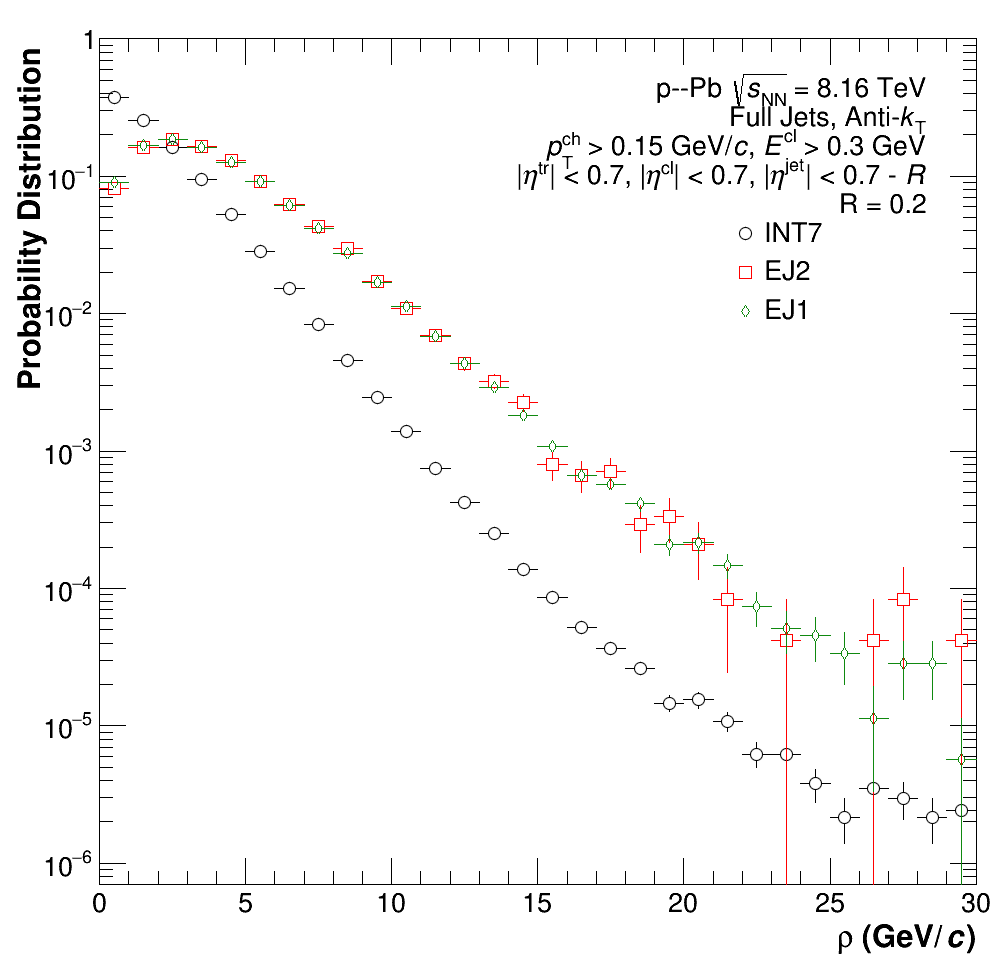
\includegraphics[width=0.49\textwidth]{figures/pPbFigures/BGSubtraction/plotRho_R02.png}
  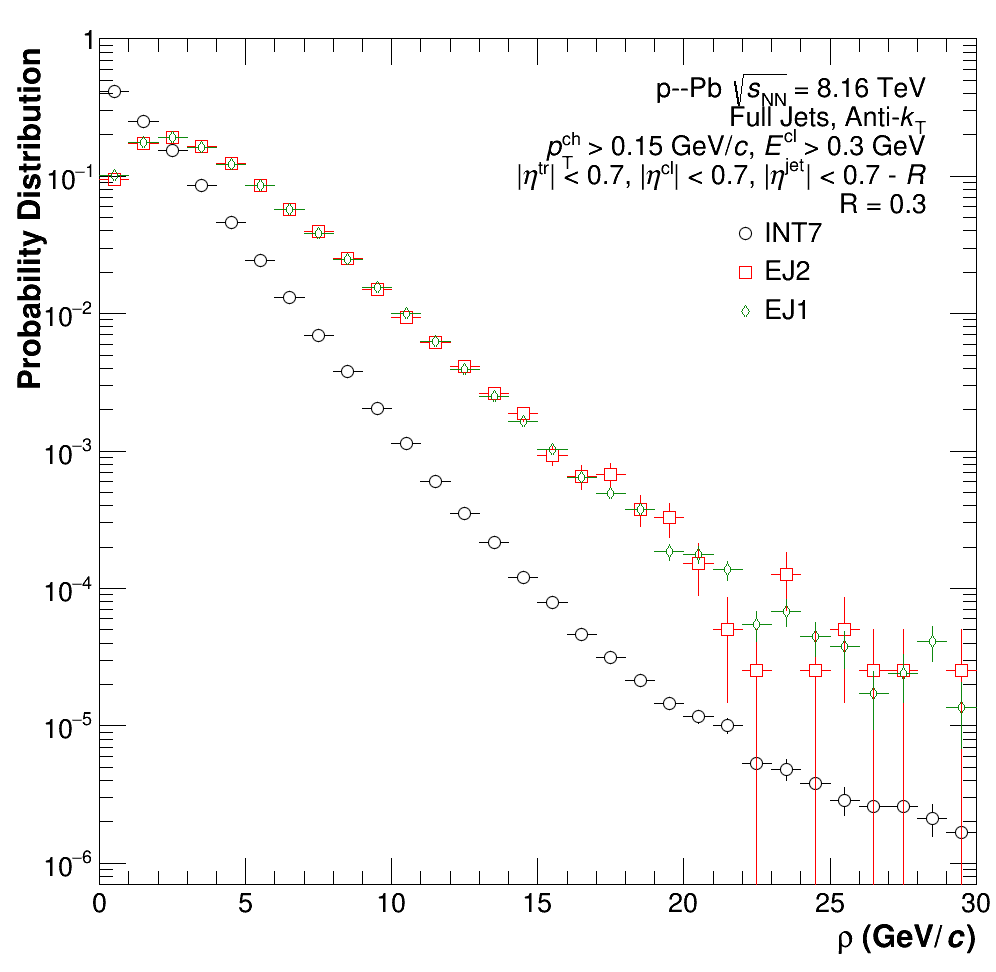
\includegraphics[width=0.49\textwidth]{figures/pPbFigures/BGSubtraction/plotRho_R03.png}
  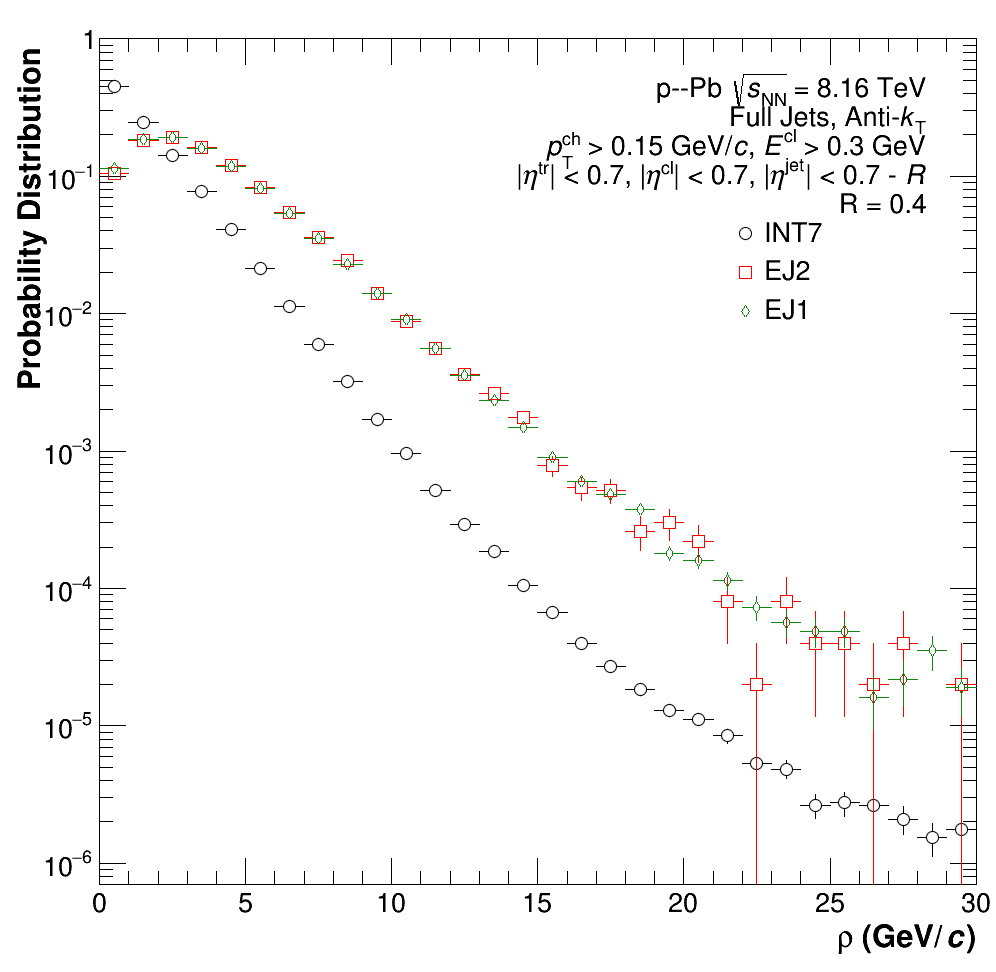
\includegraphics[width=0.49\textwidth]{figures/pPbFigures/BGSubtraction/plotRho_R04.png}
  \caption{Rho distribution for the INT7, EJ2, and EJ1 triggers in \pPb collisions for jets with resolution parameter $R$ = 0.2, 0.3, and 0.4.}
  \label{fig:Rho_distribution}
\end{figure}

The corrected jet momentum is then calculated as 

\begin{equation}
    \text{\pT}_{,jet}^{\text{corr}} = \text{\pT}_{,jet}^{\text{raw}} - \rho_{\text{CMS}} \cdot A_{\text{jet}}.
\end{equation}

\noindent
The background is calculated on an event-by-event basis using only particles within the jet acceptance and assumes a uniform background density. The true background density for each jet fluctuates around this average background density. This effect of background fluctuations is accounted for during the unfolding procedure by first using the random cones approach~\cite{ALICE:2012nbx} to find the $\delta$-\pT distribution. A cone with resolution parameter equivalent to the jet resolution parameter is randomly placed inside the $\eta-\phi$ acceptance of each event. The cone cannot overlap with the highest momentum jet and must be contained within the jet acceptance. The background fluctuations are then defined as 

\begin{equation}
    \delta \text{\pT} = \text{\pT}_\text{,RC} - \rho_{\text{CMS}} \pi R_{\text{cone}}^2
\end{equation}

\noindent
where $\text{\pT}_\text{,RC}$ is the \pT of the random cone and $R_{\text{cone}}$ is its resolution parameter. The $\delta$-\pT distribution for all three triggers is shown in Figure~\ref{fig:DeltaPt_distribution} for jets with resolution parameter $R$ = 0.2, 0.3, and 0.4. The distribution for INT7 is used since this is where the background dominates. The distribution is centered at zero with a steep tail toward negative values caused by fluctuations from soft processes. The longer tail toward positive values originates from both background fluctuations and signal.

\begin{figure}[hbt!]
  \centering
  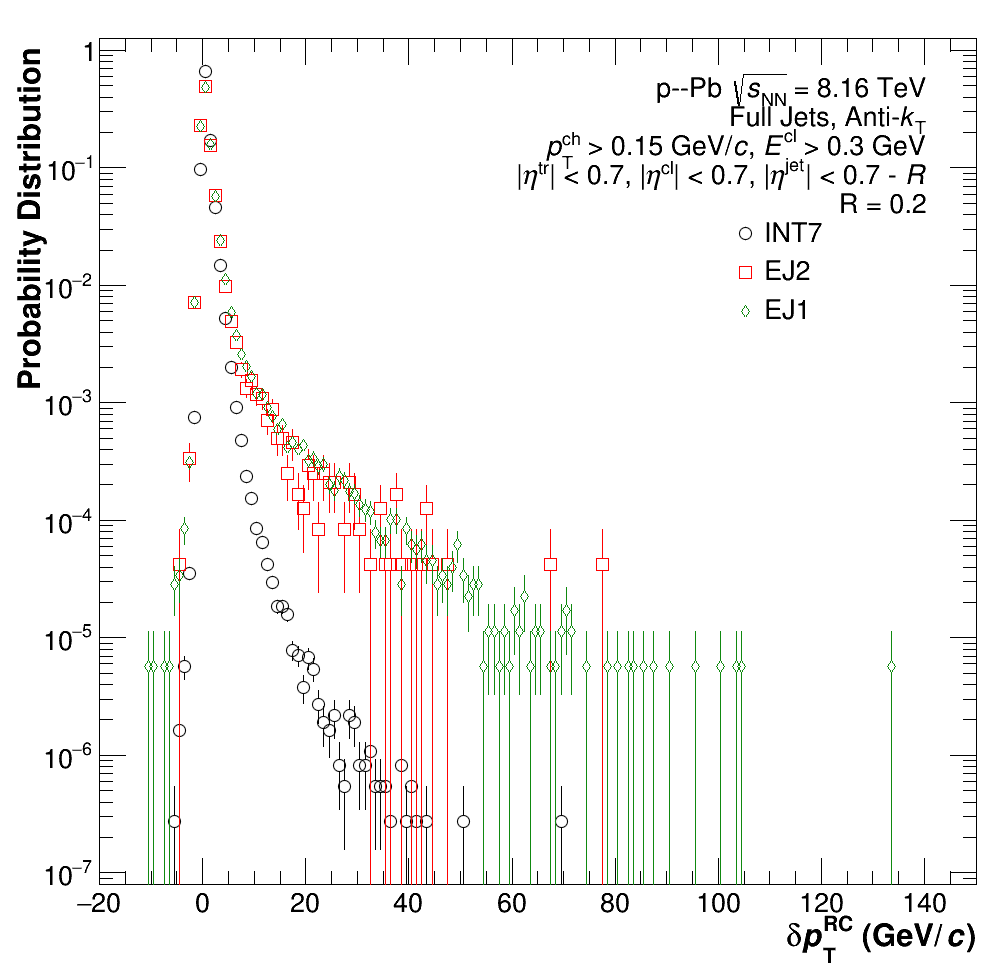
\includegraphics[width=0.49\textwidth]{figures/pPbFigures/BGSubtraction/plotDpT_R02.png}
  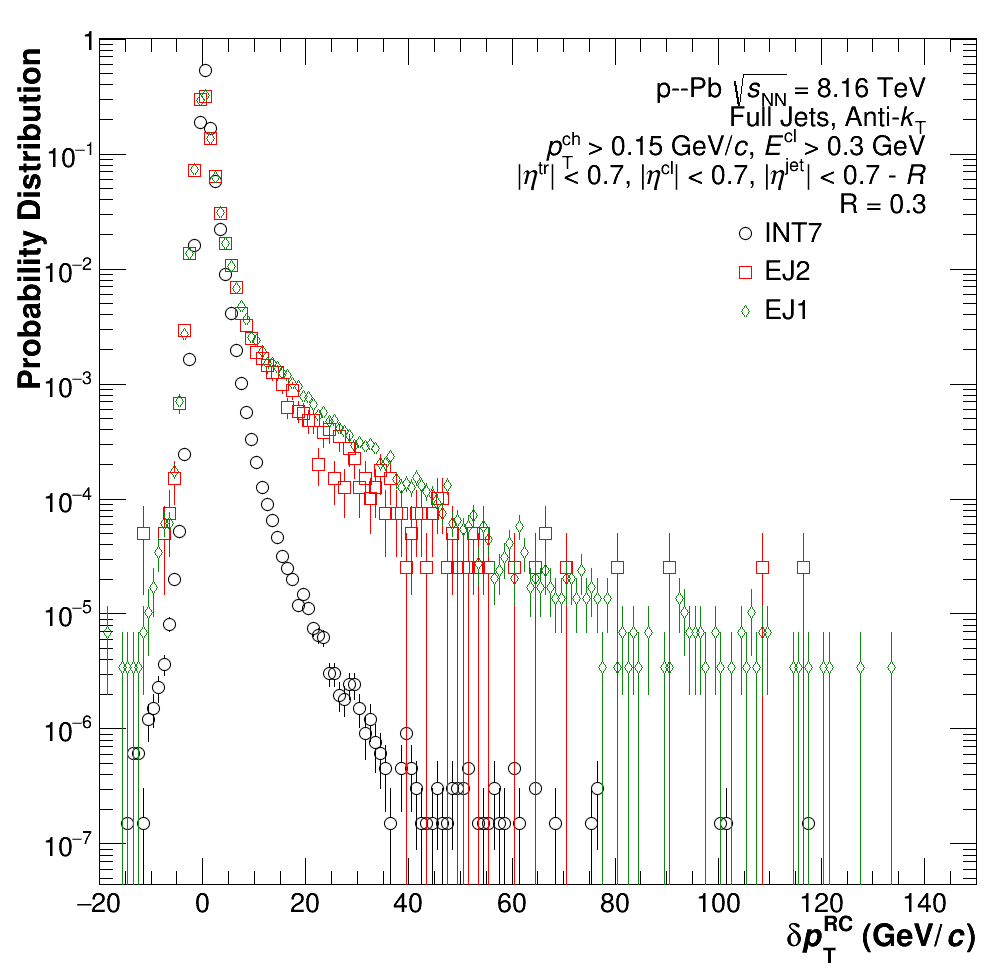
\includegraphics[width=0.49\textwidth]{figures/pPbFigures/BGSubtraction/plotDpT_R03.png}
  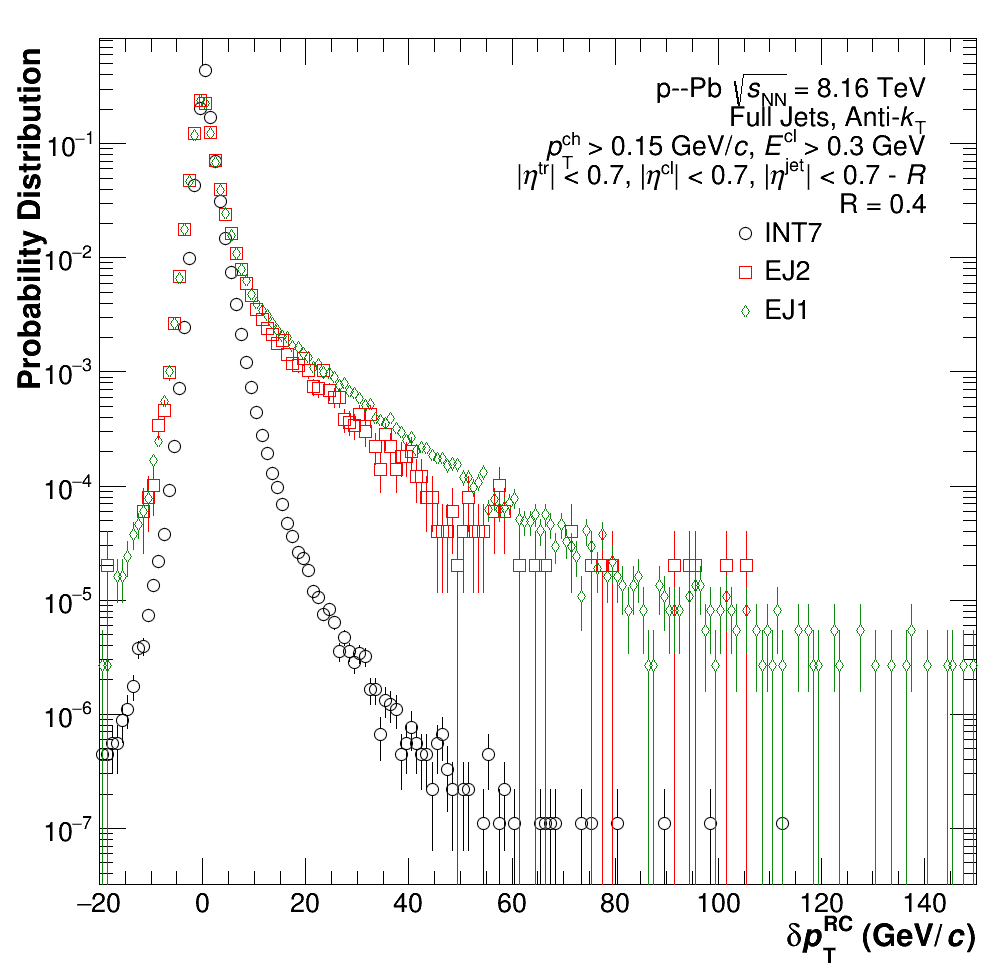
\includegraphics[width=0.49\textwidth]{figures/pPbFigures/BGSubtraction/plotDpT_R04.png}
  \caption{$\delta$-\pT distribution for the INT7, EJ2, and EJ1 triggers in \pPb collisions for jets with resolution parameter $R$ = 0.2, 0.3, and 0.4.}
  \label{fig:DeltaPt_distribution}
\end{figure}

\subsection{Trigger normalization and correction for the rejection factor}
\label{sec:triggerCorrection}

\begin{figure}
    \centering
    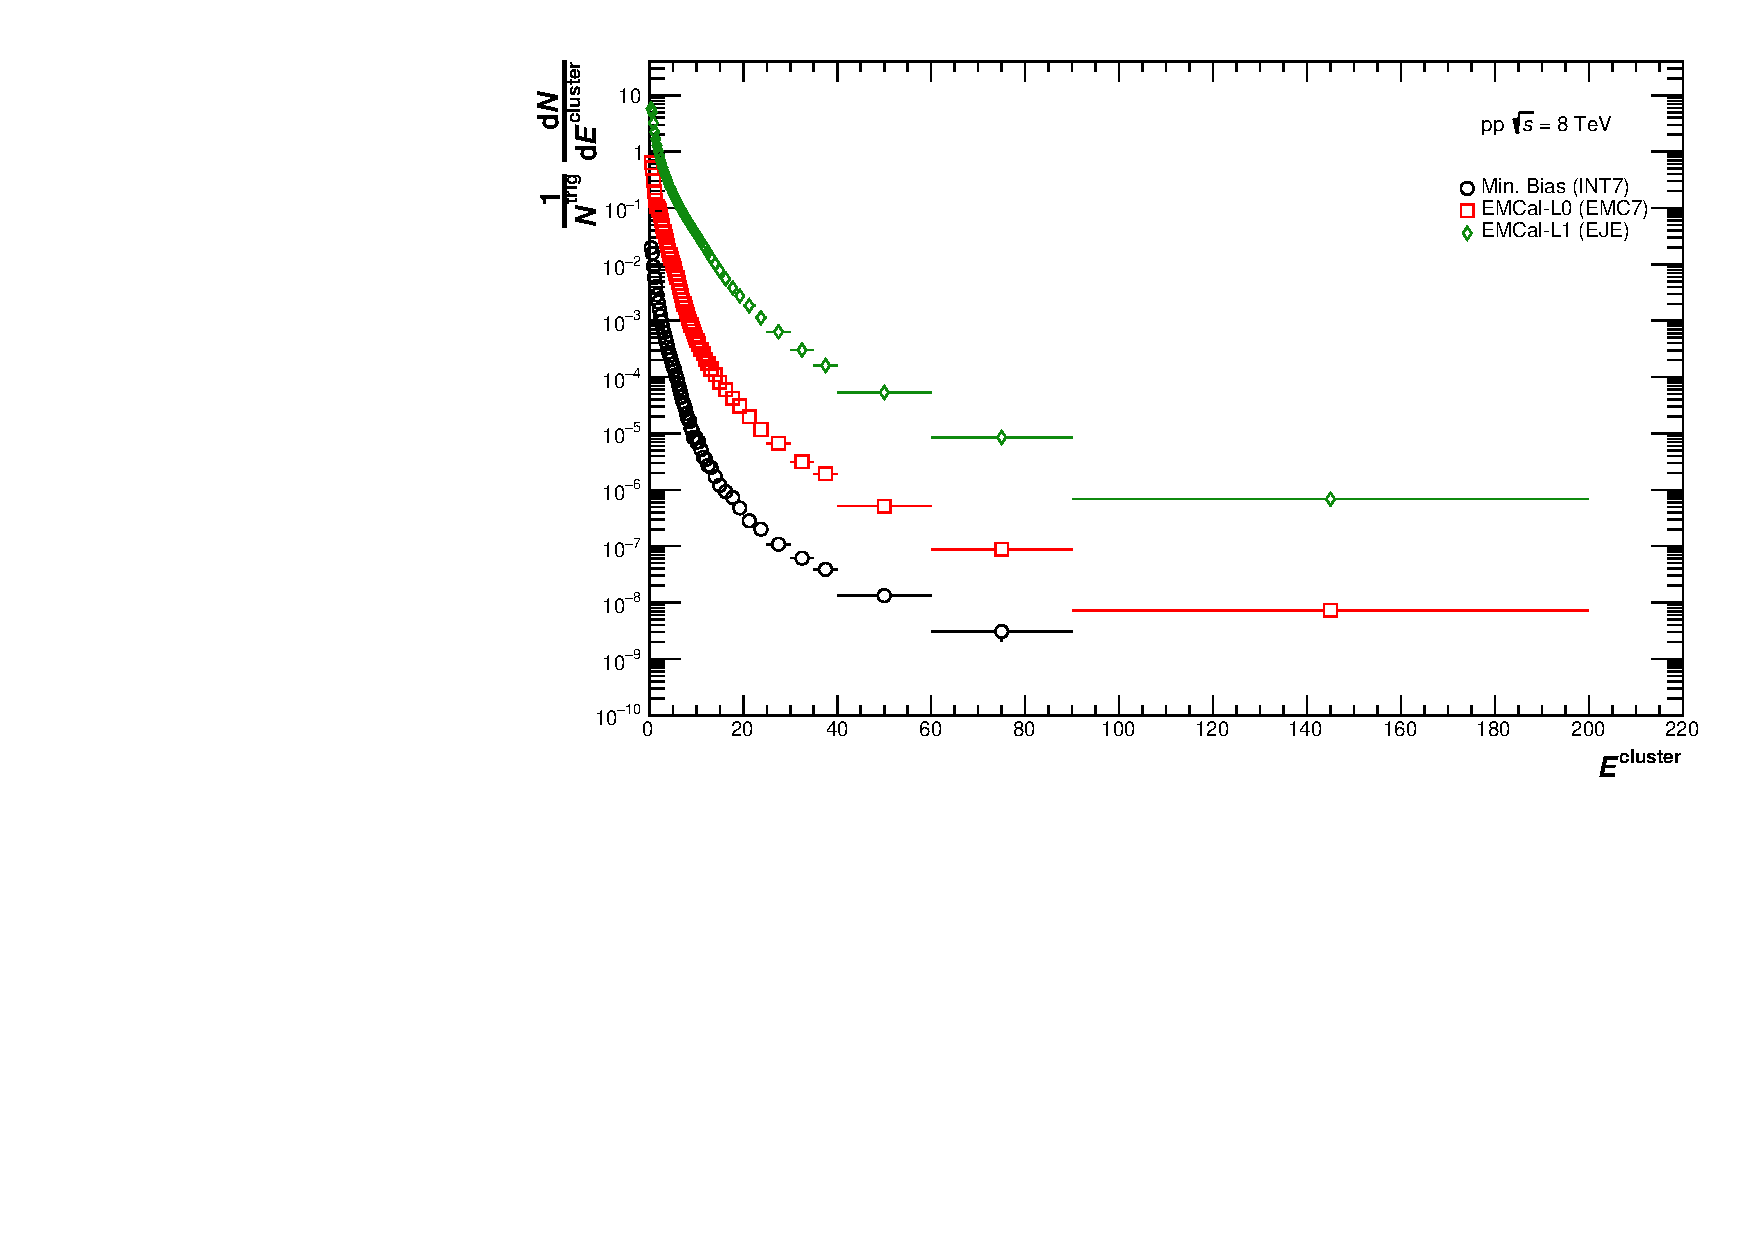
\includegraphics[width=15cm]{figures/TriggerClusters/clusters_R02.pdf}
    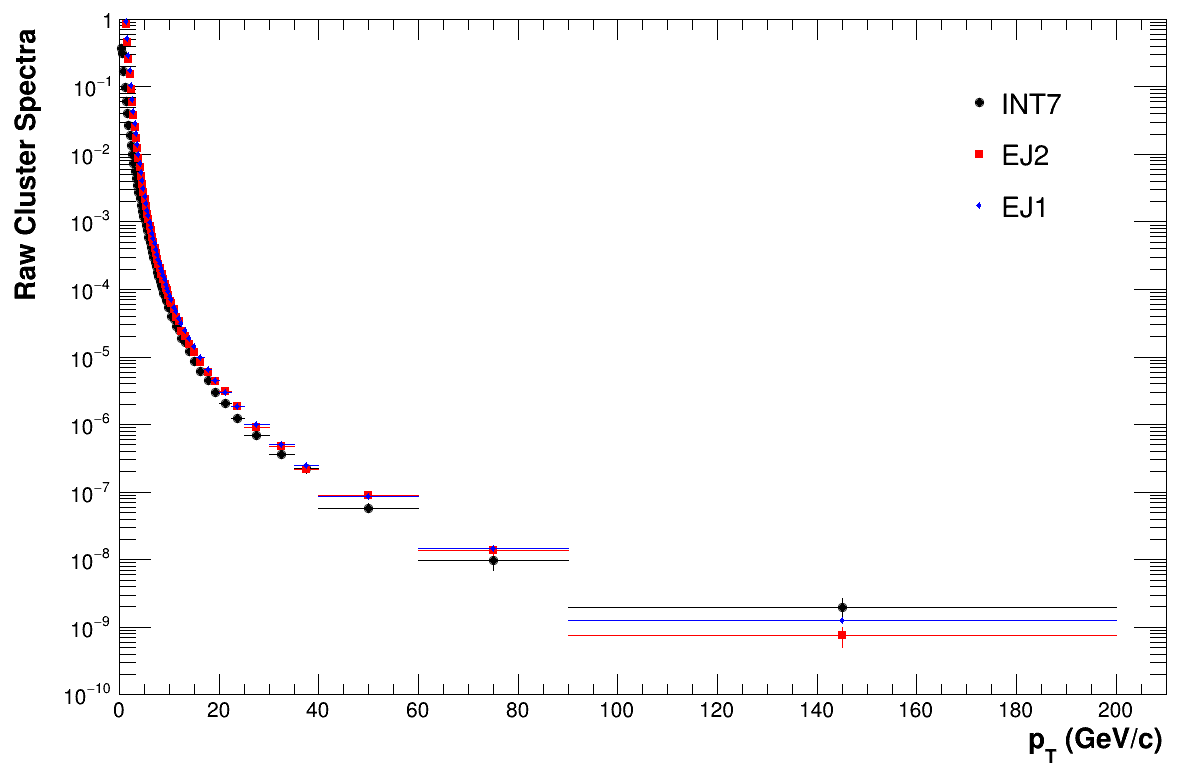
\includegraphics[width=15cm]{figures/pPbFigures/TriggerClusters/rawclusterspectra_alltriggers_R02.png}
    \caption{Trigger cluster yields for the INT7, EMC7, and EJE triggers in \pp (left), and for INT7, EJ2, and EJ1 triggers in \pPb (right). Scaling is required in order for the spectra to overlap.}
    \label{fig:triggerClusters}
\end{figure}

The trigger cluster yield for all three triggers for jet radius R = 0.2 can be found in \ref{fig:triggerClusters}. The integrated luminosity inspected by the trigger is independent of the probe, therefore it is sufficient to study only one jet radius. From this, it can be seen that the yields do not overlap. This is due to the downscaling of the minimum bias, EMC7, and EJ2 triggers (to different degrees) in order to allow trigger time for the EMCal triggers to record rare events (jets, in this case). In the 2012 dataset, these downscale factors were not recorded. Instead, the triggered data must be corrected by the use of rejection factors. These trigger rejection factors are calculated by taking the ratio of the trigger cluster yield between triggers with neighboring thresholds after correction for the cluster trigger efficiency. In this case, the ratio is taken between the EMC7 and INT7 triggers and between the EJE and EMC7 triggers. The EMC7 trigger is then divided by the former, while the EJE trigger is divided by both rejection factors. The ratio of cluster yields for different triggers without correction for the cluster trigger efficiency is shown in figure \ref{fig:RejectionFactorsUnscaled}. The plateaus are fit with an error function, and the flat region of the function is taken as the constant rejection factor. The ratio of cluster yields for different triggers after the trigger efficiency correction is shown in figure \ref{fig:RejectionFactors}. The plateaus are fit linearly to find the rejection factor.

\begin{figure}
    \centering
    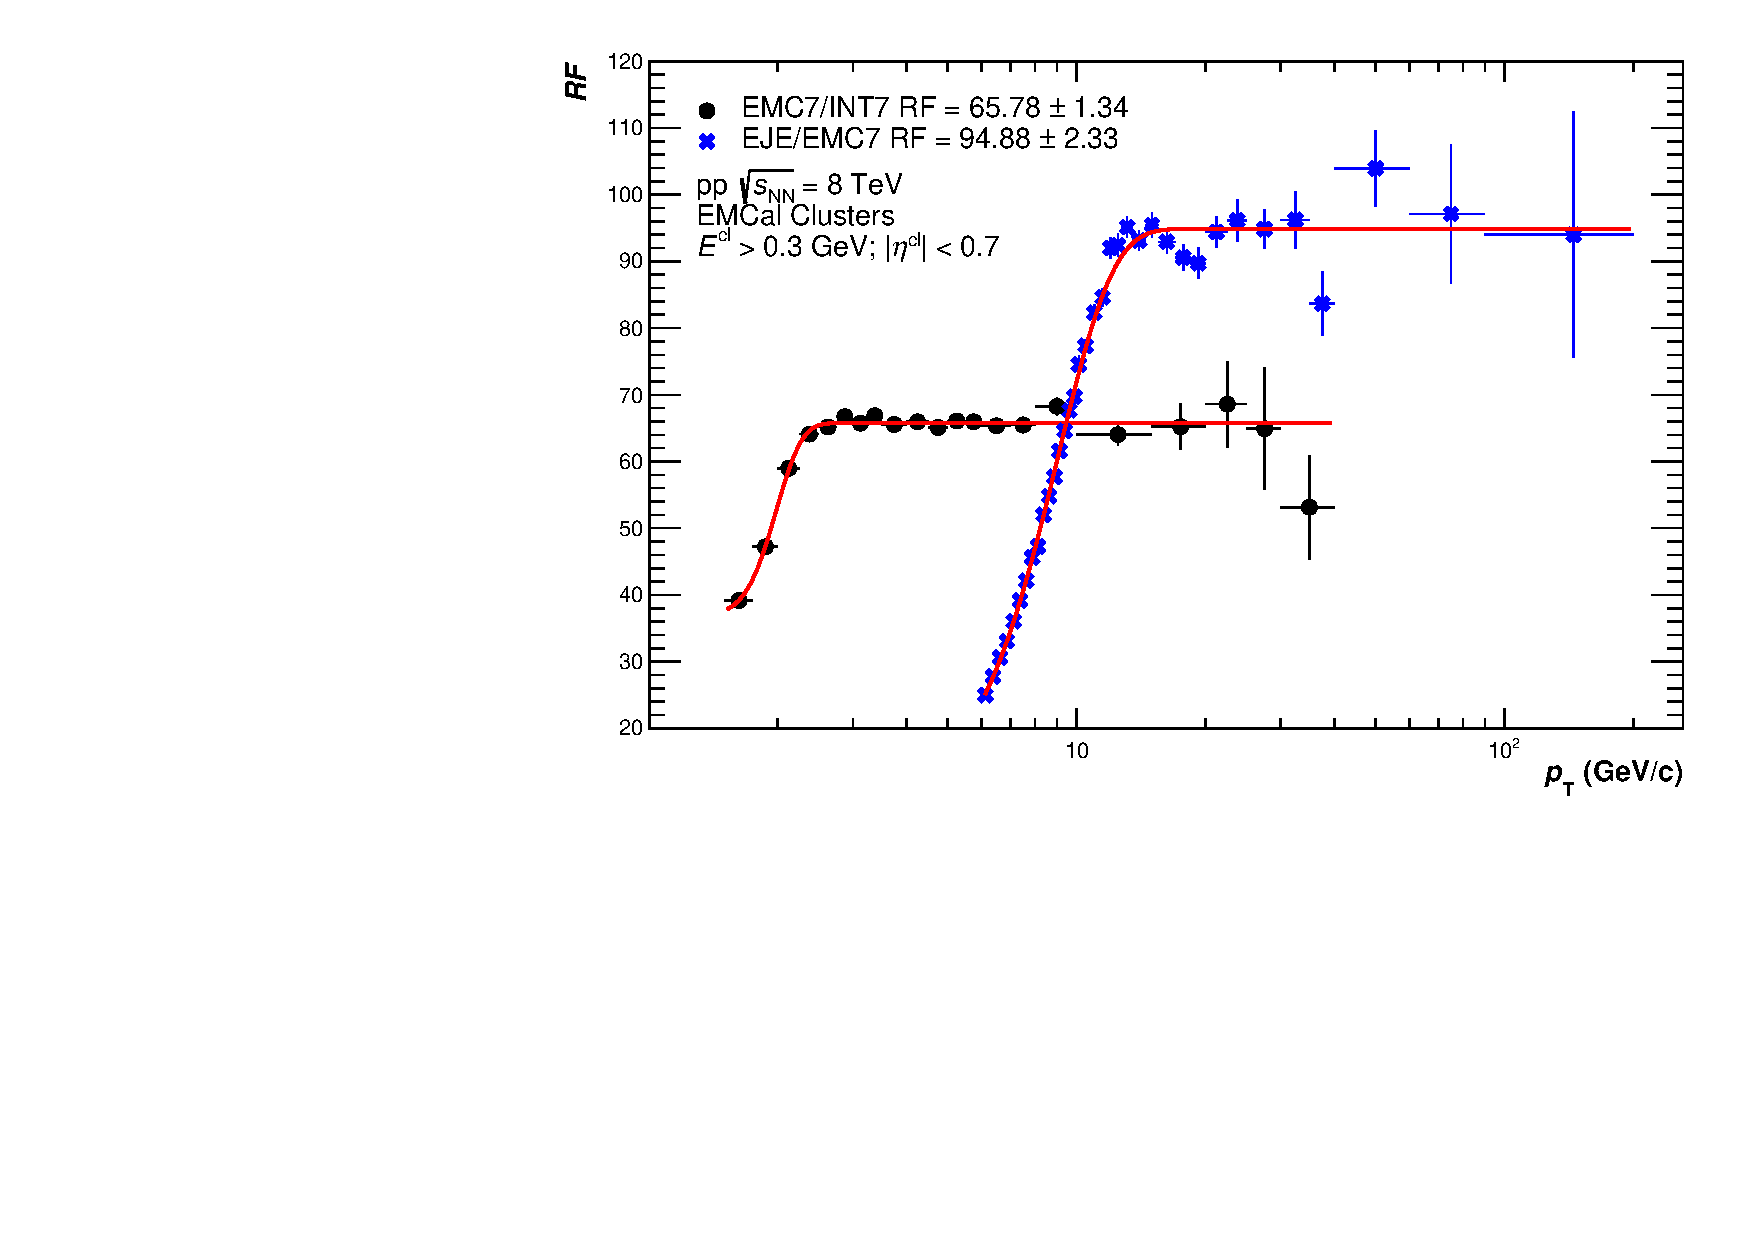
\includegraphics[width=15cm]{figures/RejectionFactors/RF_R02_Unscaled.pdf}
    \caption{Rejection factors for the EMC7 trigger and the EJE trigger, found by taking the ratio of the event-normalized trigger yields of the EMC7/INT7 triggers and EJE/EMC7 triggers, respectively.}
    \label{fig:RejectionFactorsUnscaled}
\end{figure}

\begin{figure}
    \centering
    \includegraphics[width=15cm]{figures/RejectionFactors/RF_R02.pdf}
    \caption{Rejection factors scaled by the cluster trigger efficiency in \pp.}
    \label{fig:RejectionFactors}
\end{figure}

In the \pPb dataset, the observed, integrated luminosity can be used to scale the spectra in place of the rejection factors. The trigger setup is configured in trigger clusters, which contain a set of detectors read out at once. The time the detector is live is determined by the slowest detector in the cluster, so if you remove that, you can take more collisions. If you have triggers in different clusters, the livetime can be different, which must be corrected for. There is typically at least one trigger shared by two clusters that can be used to compare them and find corrections. Because the corrections factorize, the integrated luminosity of the trigger can be calculated based on the event count and the downscaling of the min. bias trigger.

\subsection{Combination of the triggers at raw level}
\label{sec:triggerCombination}

\begin{figure}
    \centering
    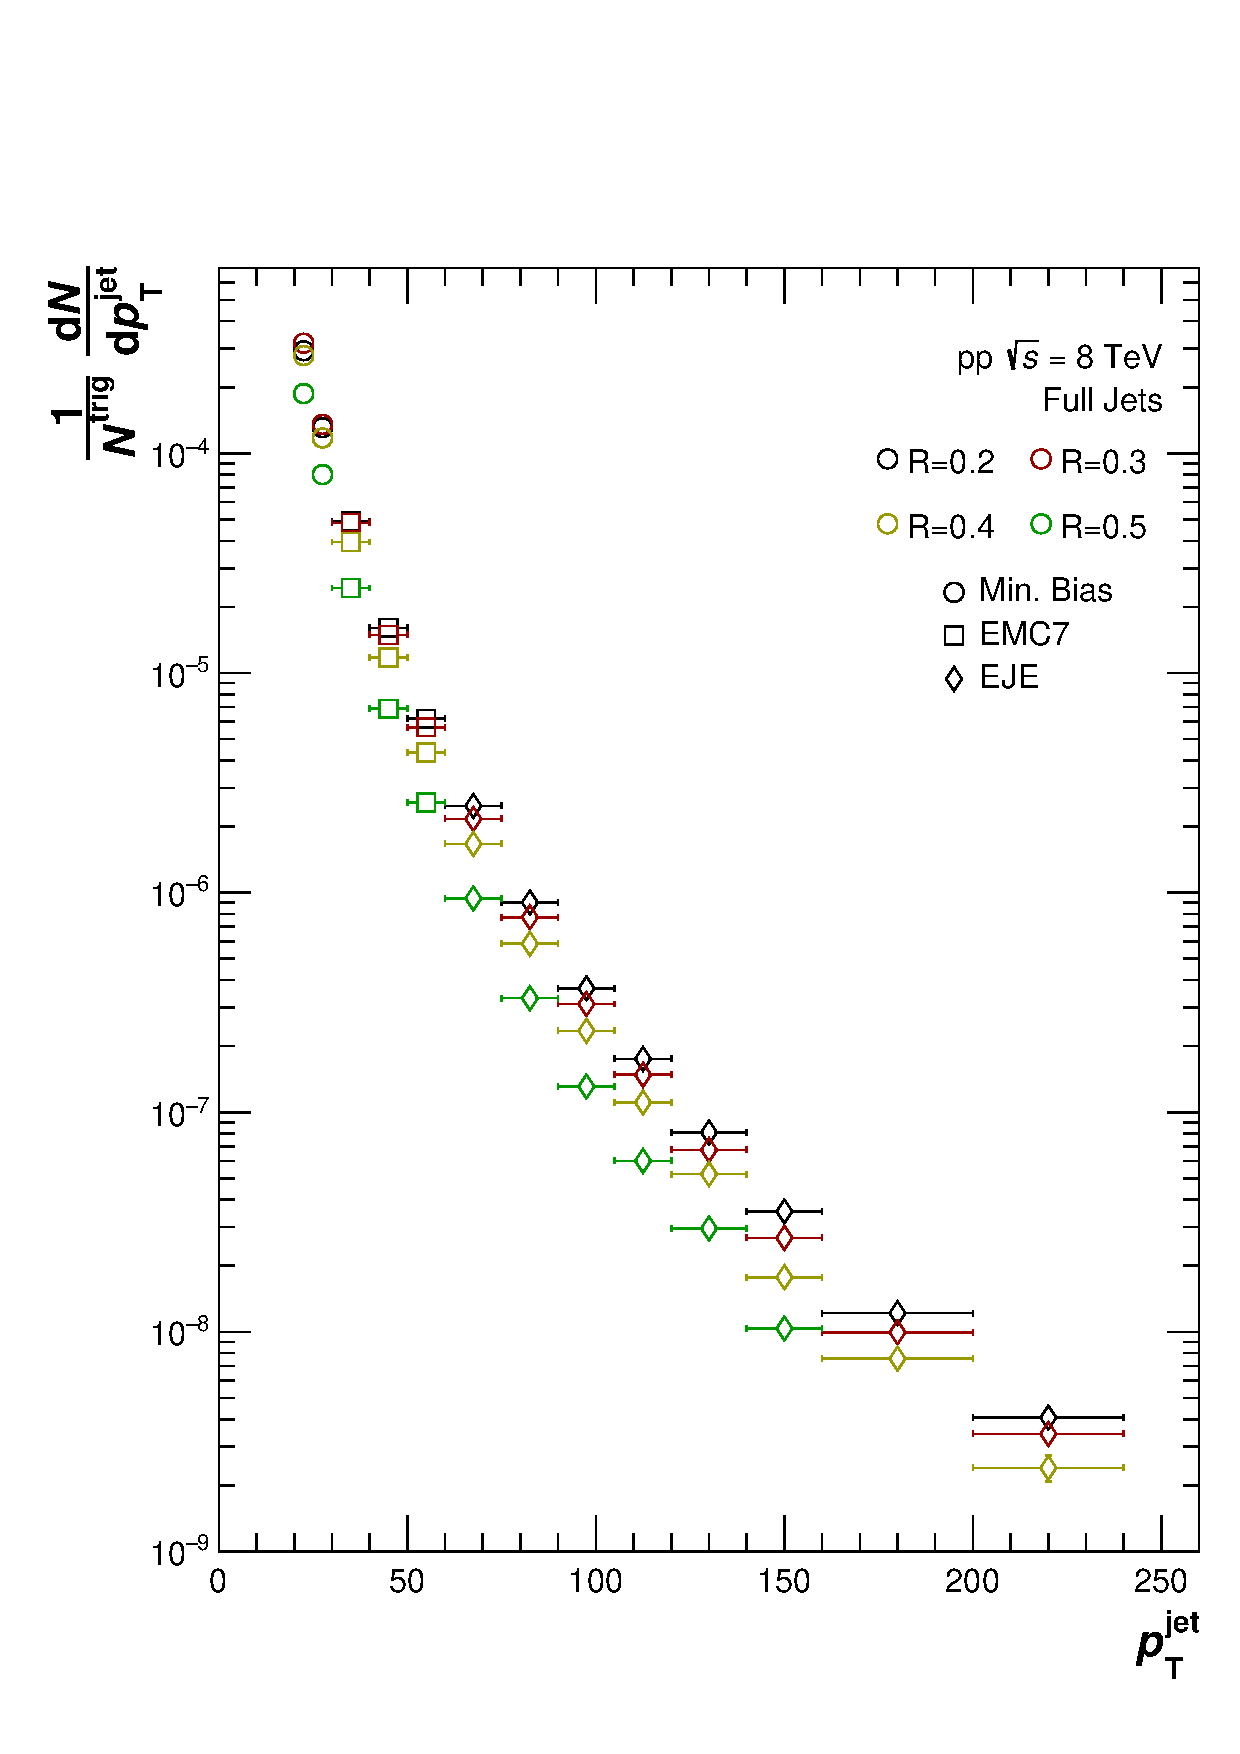
\includegraphics[width=7.5cm]{figures/CorrRawSpec/corrRawSpec.pdf}
    \caption{Raw spectra for the three triggers with corrections from chapter \ref{chap:TriggerAndInstrumentation} for varous jet radii.}
    \label{fig:CorrRawSpec}
\end{figure}

The raw spectrum is constructed by combining the raw spectra from the three trigger classes after the application of the rejection factors and the corrections discussed in chapter \ref{chap:TriggerAndInstrumentation}. Fig. \ref{fig:CorrRawSpec} shows the comparison of the raw spectra from the three triggers in \pp for jets with different jet radii. 

As can be seen in section \ref{sec:EMCTriggerBias}, figure \ref{fig:trigger_ratios}, the ratio EMC7/INT7 (EJE/EMC7) deviates from 1 for jets with pt $>$ 30 (60) GeV/c. As discussed in chapter \ref{sec:EMCTriggerBias}, jets with \pT $<$ 30 (60) GeV/c for the the EMC7 (EJE) trigger also suffer from effects like random noise, which are not simulated, contributing to triggers selecting jets in the sub-threshold region. The trigger efficiency is therefore underestimated in this \pT region and the corrections cannot be trusted any more. For the combination of the spectra at raw level, the data points from the triggers are selected in a way that contributes the least to the statistical uncertainty. The ranges are selected as the following:

\begin{itemize}
    \item 20 GeV/c $\le$ \pT $<$ 30 GeV/c: INT7 trigger
    \item 30 GeV/c $\le$ \pT $<$ 60 GeV/c: EMC7 trigger
    \item \pT $\ge$ 60 GeV/c: EJE trigger
\end{itemize}

These ranges are chosen based on the topics discussed in section \ref{sec:ptRanges}. Additionally, at very high momentum, energy corrections - in particular with respect to the non-linearity in EMCal - are not sufficiently well understood to perform a measurement.

The same is true for the triggers in \pPb, and the ranges for these triggers are selected as the following:

\begin{itemize}
    \item 20 GeV/c $\le$ \pT $<$ 30 GeV/c: INT7 trigger
    \item 30 GeV/c $\le$ \pT $<$ 50 GeV/c: EJ2 trigger
    \item \pT $\ge$ 50 GeV/c: EJ1 trigger
\end{itemize}

\subsection{Cross section normalization}
\label{sec:xsecNomalization}

Since the jet yield was measured only in the EMCal acceptance, a correction for the limited acceptance has to be applied. The acceptance correction is

\begin{equation}
    Acc = \frac{\Delta\eta \Delta\phi}{2\pi}
\end{equation}

where $\Delta\eta$ = 1.4 − 2R and $\Delta\phi$ = 1.745 − 2R for \pp, and $\Delta\eta$ = 1.4 − 2R and $\Delta\phi$ = 1.887 − 2R for \pPb. The phi correction is different for the \pPb dataset because extra EMCal modules were added during long shutdown 1, between run 1 and run 2.

The number of events has to be corrected for the vertex finding efficiency. The vertex finding efficiency is defined as the fraction of events before and after vertex selection and is evaluated before the vertex-z cut. The vertex finding efficiency has been determined from the event counters for accepted and rejected events to be 94.8$\%$ for INT7, 99.2$\%$ for EMC7, and 99.6$\%$ for EJE, and applied as scaling factor to the spectrum. EMCal triggered events have a higher multiplicity on average, so there are more tracks to reconstruct the vertex with, especially in pp-collisions. Since luminosity scaling is used in the \pPb dataset instead of the rejection factors, the INT7 vertex finding efficiency is used for all triggers. EMCal triggers are a biased subsample of INT7, which have nearly 100\% vertex finding efficiency. Since the correction is performed to the NSD event type, the efficiency from the reference trigger (INT7) must be used, whic in this case is 98.6\%.

The reference cross section for the INT7 trigger (V0AND condition) has been determined in a van-der-Meer scan to be 55.8 mb with an uncertainty of 2.6$\%$ in \pp, and 2095 mb with an uncertainty of 1.9$\%$ in \pPb. The total correction excluding unfolding is

\begin{equation}
   \frac{d\sigma_{\pp}}{dp_T d\eta} = \frac{\sigma_{V0AND}\epsilon_{vtx}}{N_{trg,INT7}} \frac{1}{Acc\epsilon_{trg}*RF} \frac{dN_{jet}}{dp_T d\eta}
\end{equation}

\begin{equation}
   \frac{d\sigma_{\pPb}}{dp_T d\eta} = \frac{\epsilon_{vtx}}{Acc\epsilon_{trg}*L} \frac{dN_{jet}}{dp_T d\eta}
\end{equation}

with the corrected trigger yield N$_{trg,INT7}$, the vertex finding efficiency $\epsilon_{vtx}$, the trigger efficiency $\epsilon_{trg}$, and the rejection factor RF, which is 1 for the INT7 trigger. The corrected raw spectrum for different jet radii before unfolding is shown in fig. \ref{fig:CombinedRawSpec}

%\begin{figure}
%    \centering
%    \includegraphics[width=15cm]{figures/CorrRawSpec/corrRawSpec_Combined.pdf}
%    \includegraphics[width=15cm]{figures/pPbFigures/CorrRawSpec/corrRawSpec_Combined.pdf}
%    \vfill\null
%    \caption{Combined raw spectrum after corrections for the rejection factors, vertex finding efficiency, trigger efficiency, and cross-section normalization for \pp (top) and \pPb (bottom).}
%    \label{fig:CombinedRawSpec}
%\end{figure}
\textcolor{red}{I edited out a figure here. Make sure stuff lines up}

\subsection{Unfolding of the jet spectrum}
\label{sec:unfolding}
\subsubsection{Kinematic efficiency}
\label{subsec:kinEff}

\begin{figure}
    \centering
    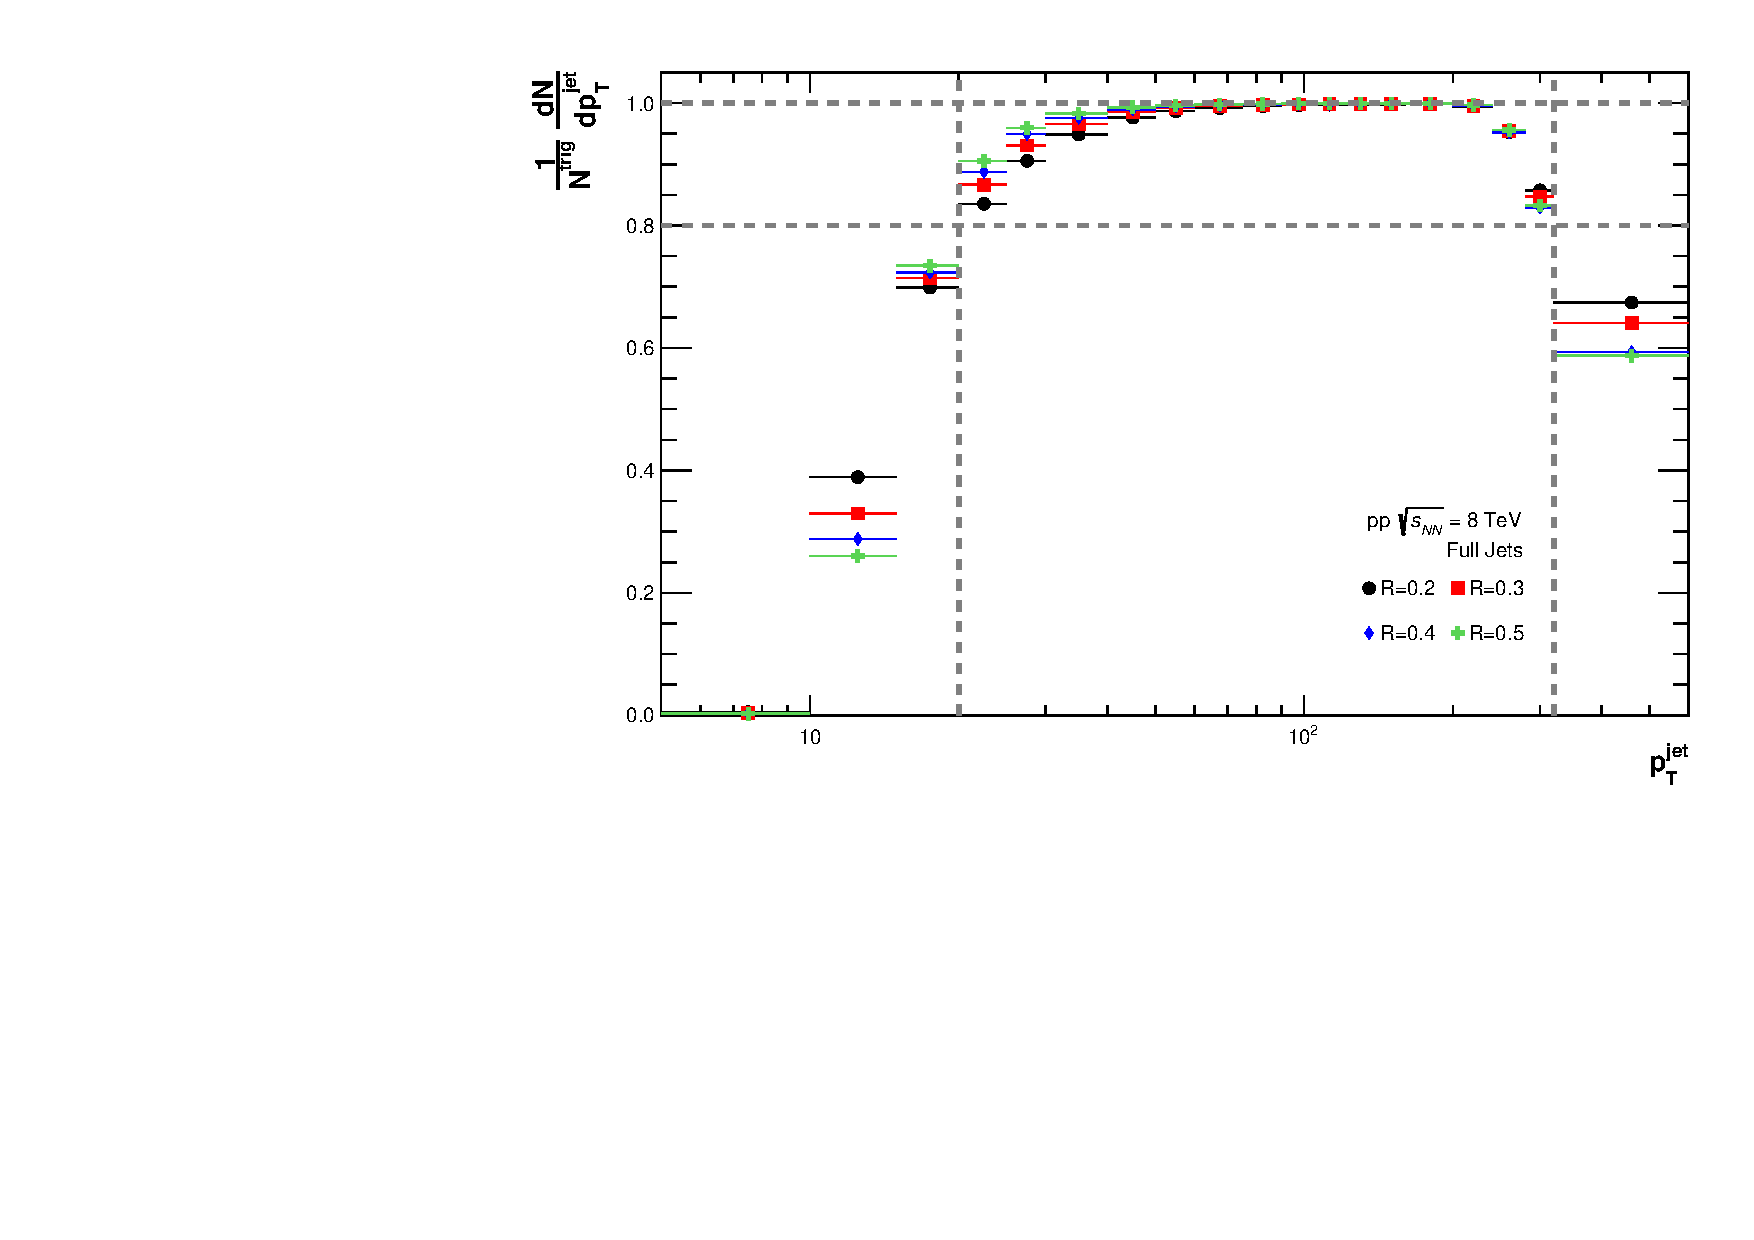
\includegraphics[width=15cm]{figures/KinematicEfficiency/EffKine.pdf}
    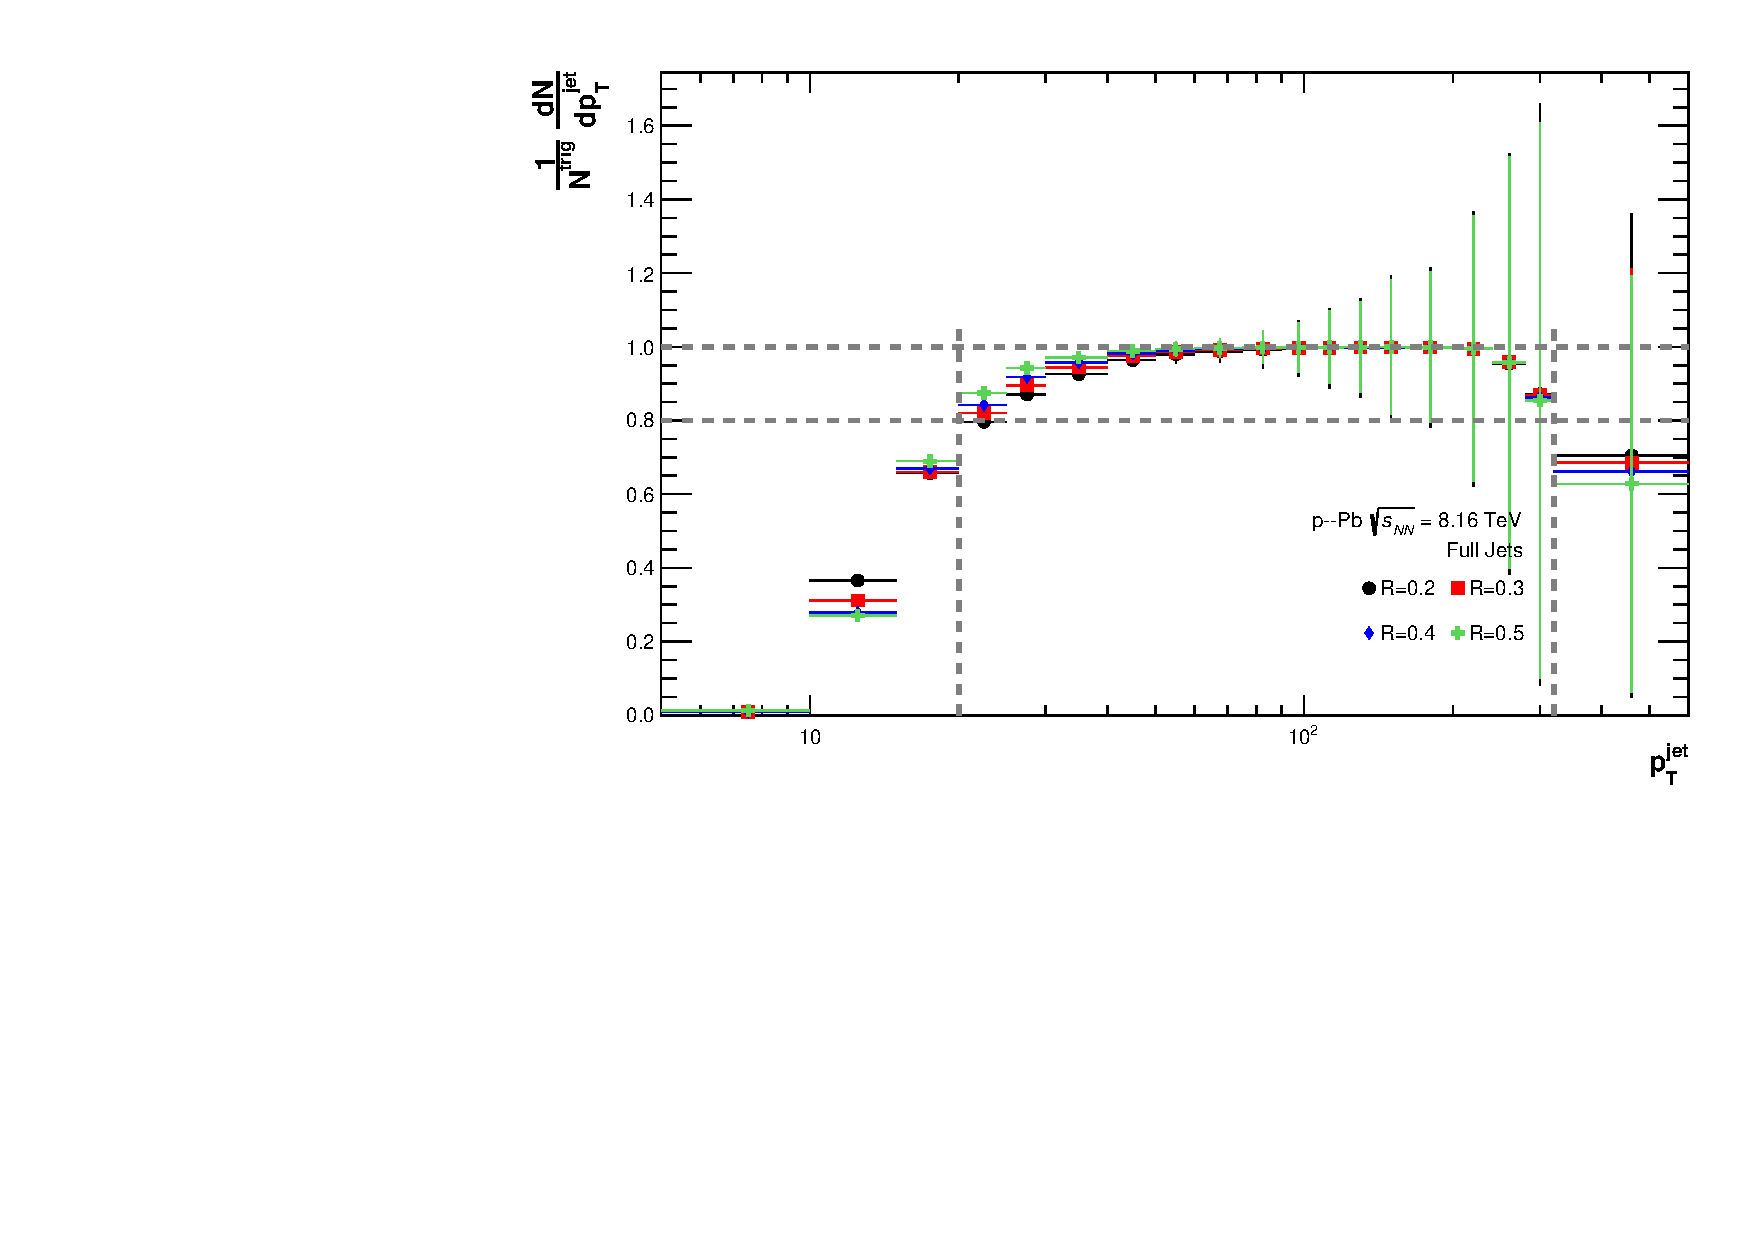
\includegraphics[width=15cm]{figures/pPbFigures/KinematicEfficiency/EffKine.pdf}
    \caption{Kinematic efficiency for various jet radii in \pp (top) and \pPb (bottom).}
    \label{fig:KinematicEfficiency}
\end{figure}

Fig. \ref{fig:KinematicEfficiency} shows the kinematic efficiency for jets with R=0.2 to R=0.6 [0.5]. Jets are selected at detector level to have a \pT within 10 and 240 GeV/c. The efficiency is 80$\%$ beyond 20 GeV/c, and stays around this value in the whole region covered by the measurement. At lower \pT, the turn-on is sharper for jets with larger jet radii. The kinematic efficiency is corrected for in the unfolding procedure. A measurement is feasible for 20 GeV /c $<$ \pT $<$ 320 GeV/c, where the reported range is selected where the kinematic efficiency is larger than 80$\%$.

\subsubsection{Unfolding tests - \pp}
\label{subsec:unfoldingTests}

For this measurement, both bayesian unfolding and unfolding based on singular value decomposition (SVD) are used. Both methods were implemented in the RooUnfold framework \cite{roounfold}. The bayesian method is used as the standard method, while SVD unfolding is used to test the sensitivity with respect to different unfolding methods. It is important to note that the unfolding procedure corrects towards harder spectra. The following figures contain test results for jet radius R = 0.2 for SVD and Bayesian unfolding. For the remaining jet radii, see appendix \ref{sec:AppendixUnfoldingTests}.

\begin{figure}
    \centering
    \begin{multicols}{2}
            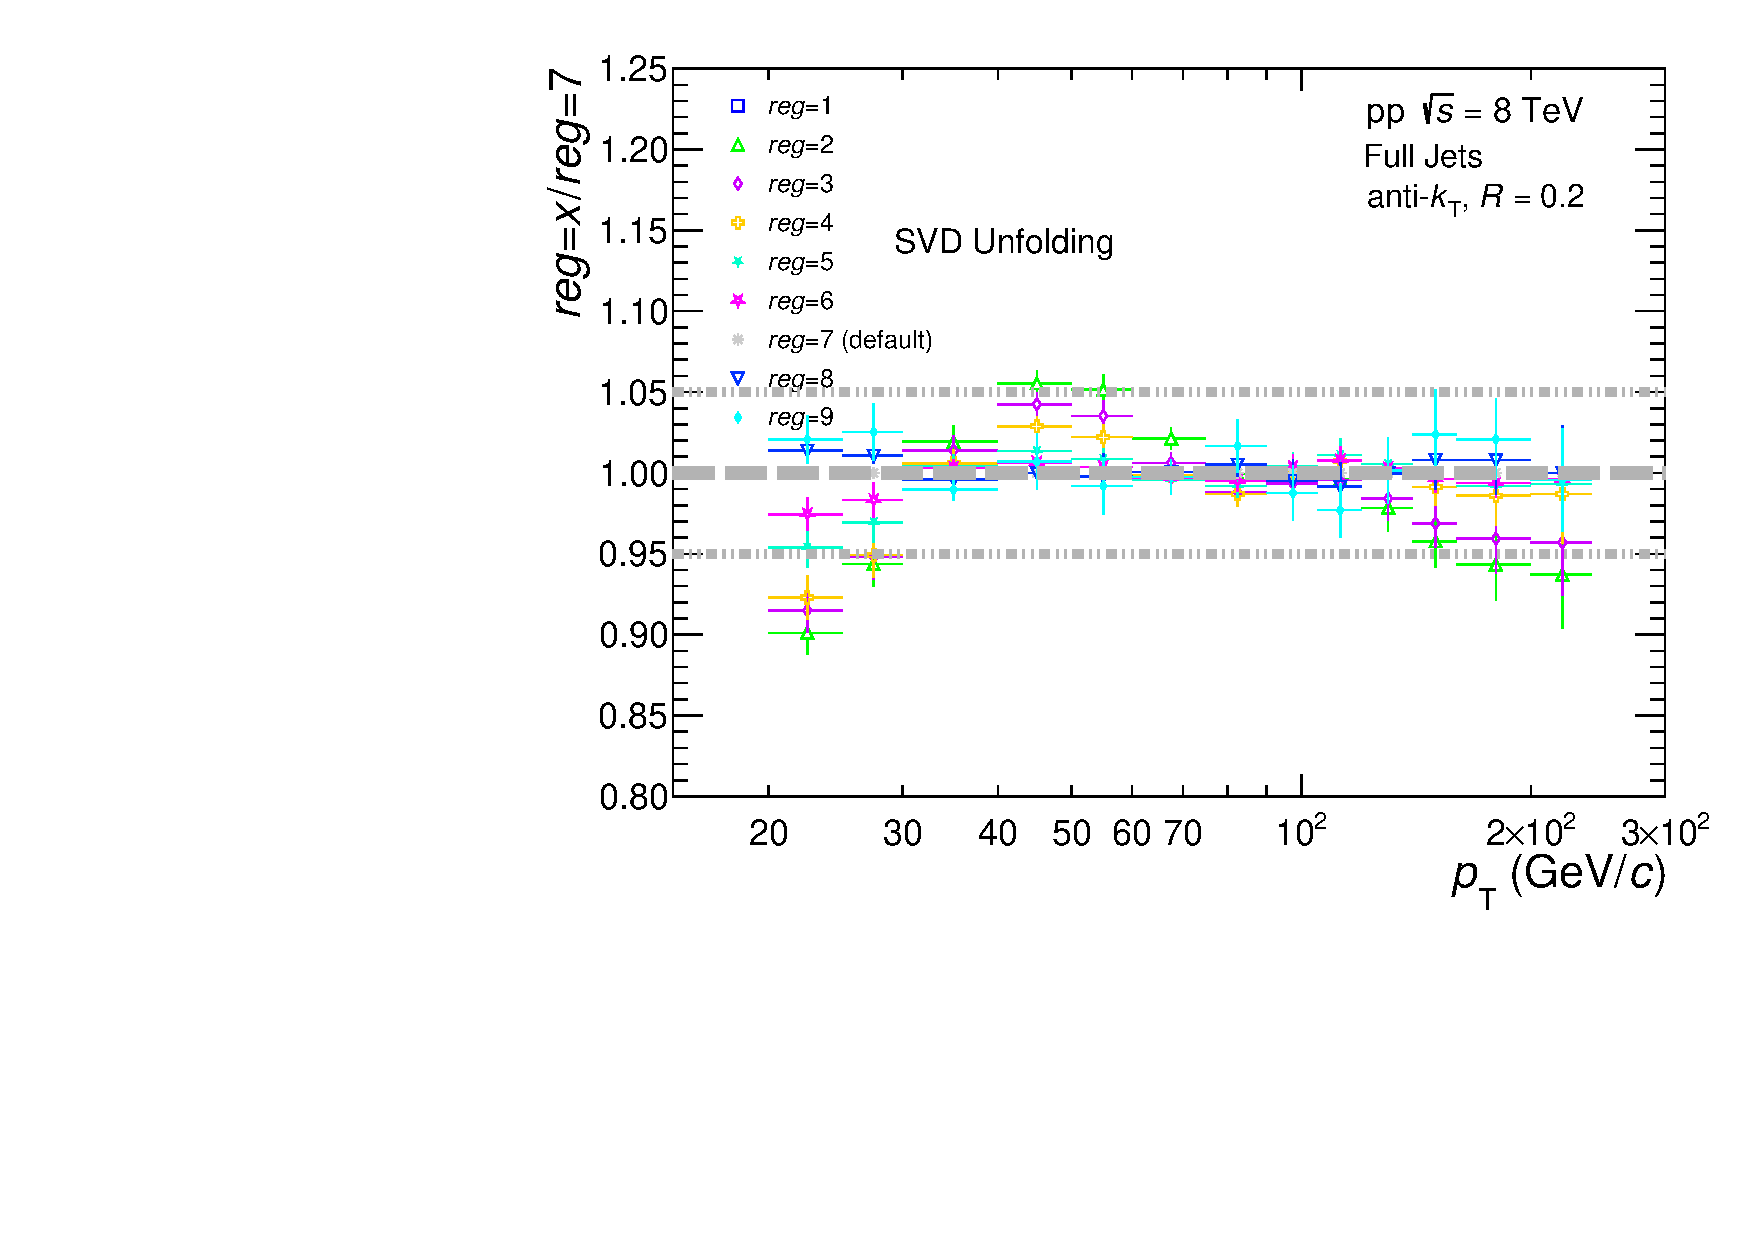
\includegraphics[width=7.5cm]{figures/UnfoldingComparisons/Regularizations/RatioRegularizationSvd_R02.pdf}
        \vfill\null 
        \columnbreak
            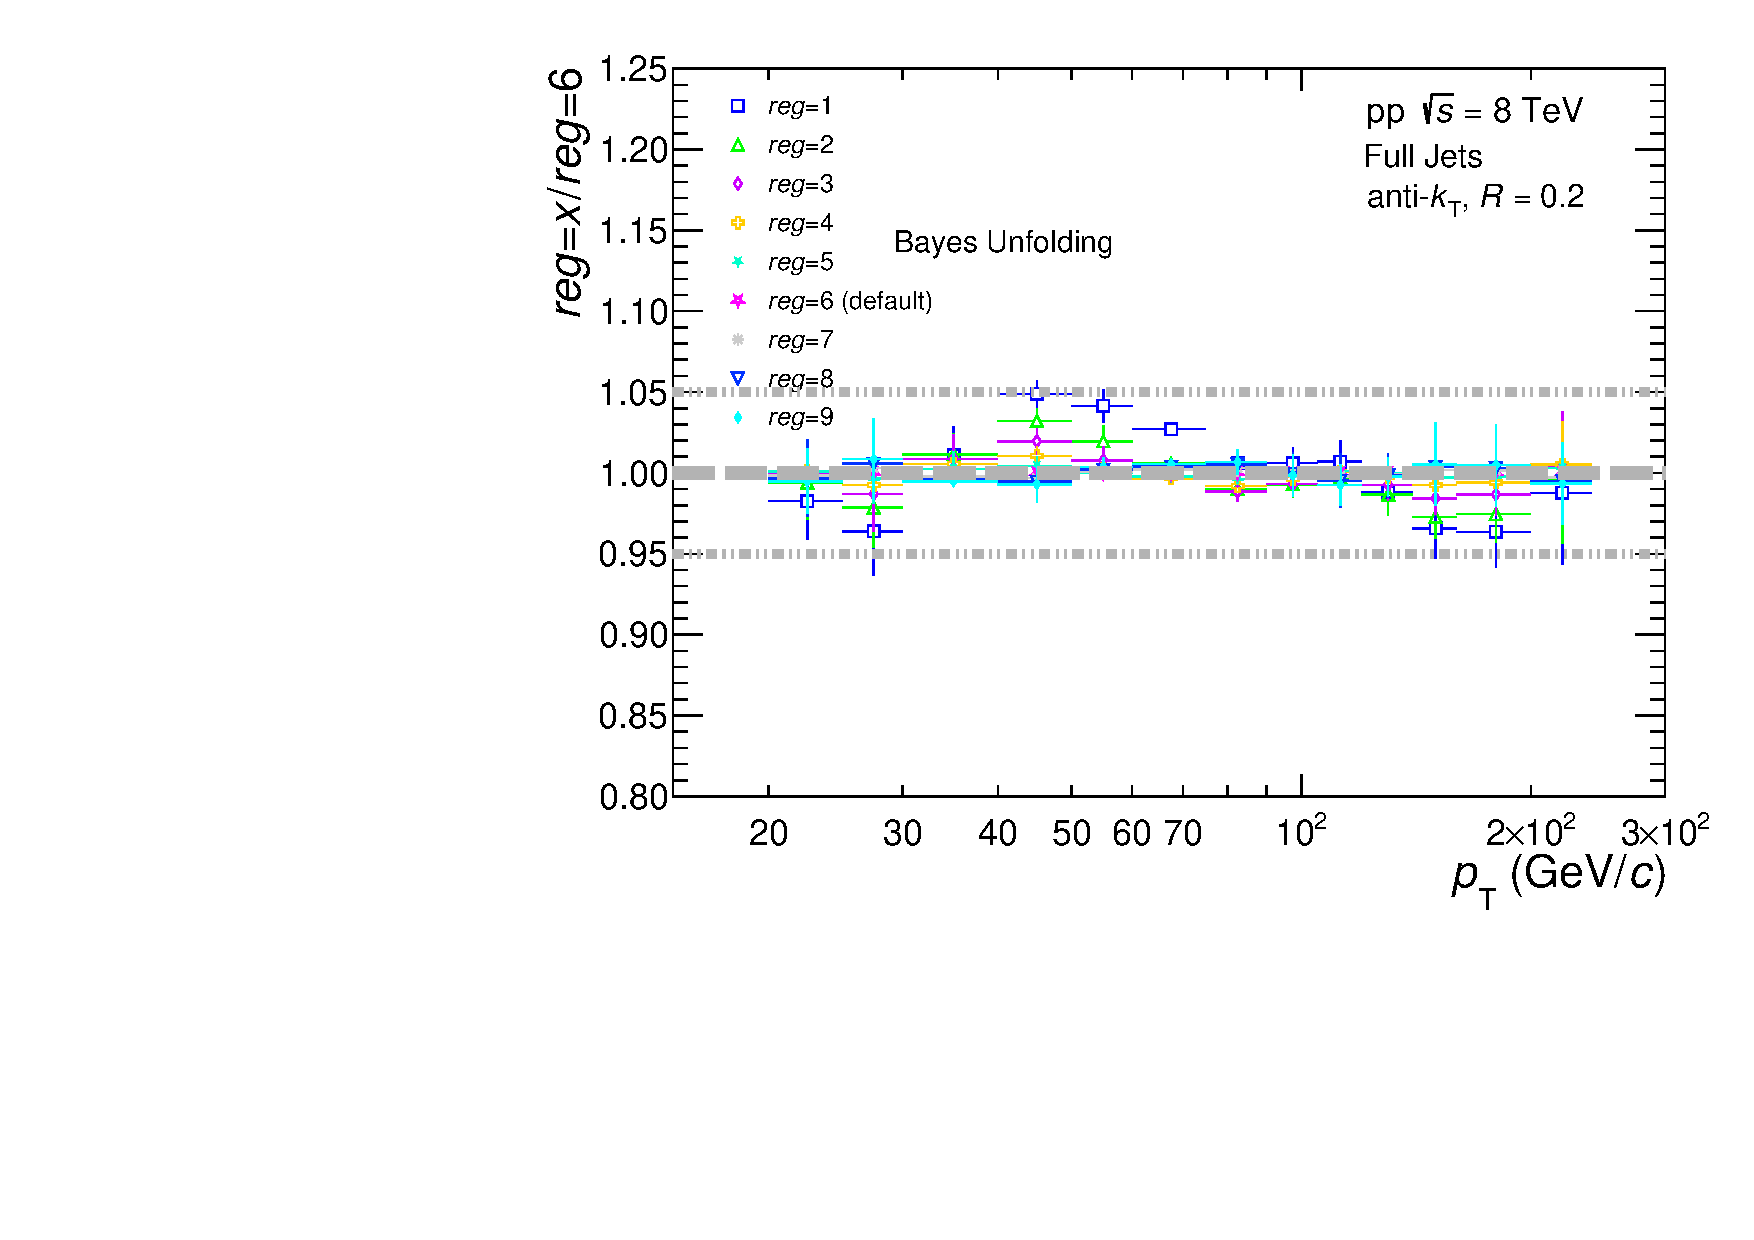
\includegraphics[width=7.5cm]{figures/UnfoldingComparisons/Regularizations/RatioRegularizationBayes_R02.pdf}
        \vfill\null
    \end{multicols}
    \caption{Regularization dependence for SVD (left) and Bayesian (right) unfolding.}
    \label{fig:RegIter}
\end{figure}

Fig. \ref{fig:RegIter} shows the dependence of the SVD and bayesian undfolded solutions on the regularization parameter. A regularization parameter of 7 is selected as default for the SVD unfolding, while for bayesian unfolding, 6 iterations is chosen as default with 4 and 9 as variations. The choice of the regularization parameter for SVD of 7 is also motivated by the D-vector (Fig. \ref{fig:DVector}). 

\begin{figure}
    \centering
    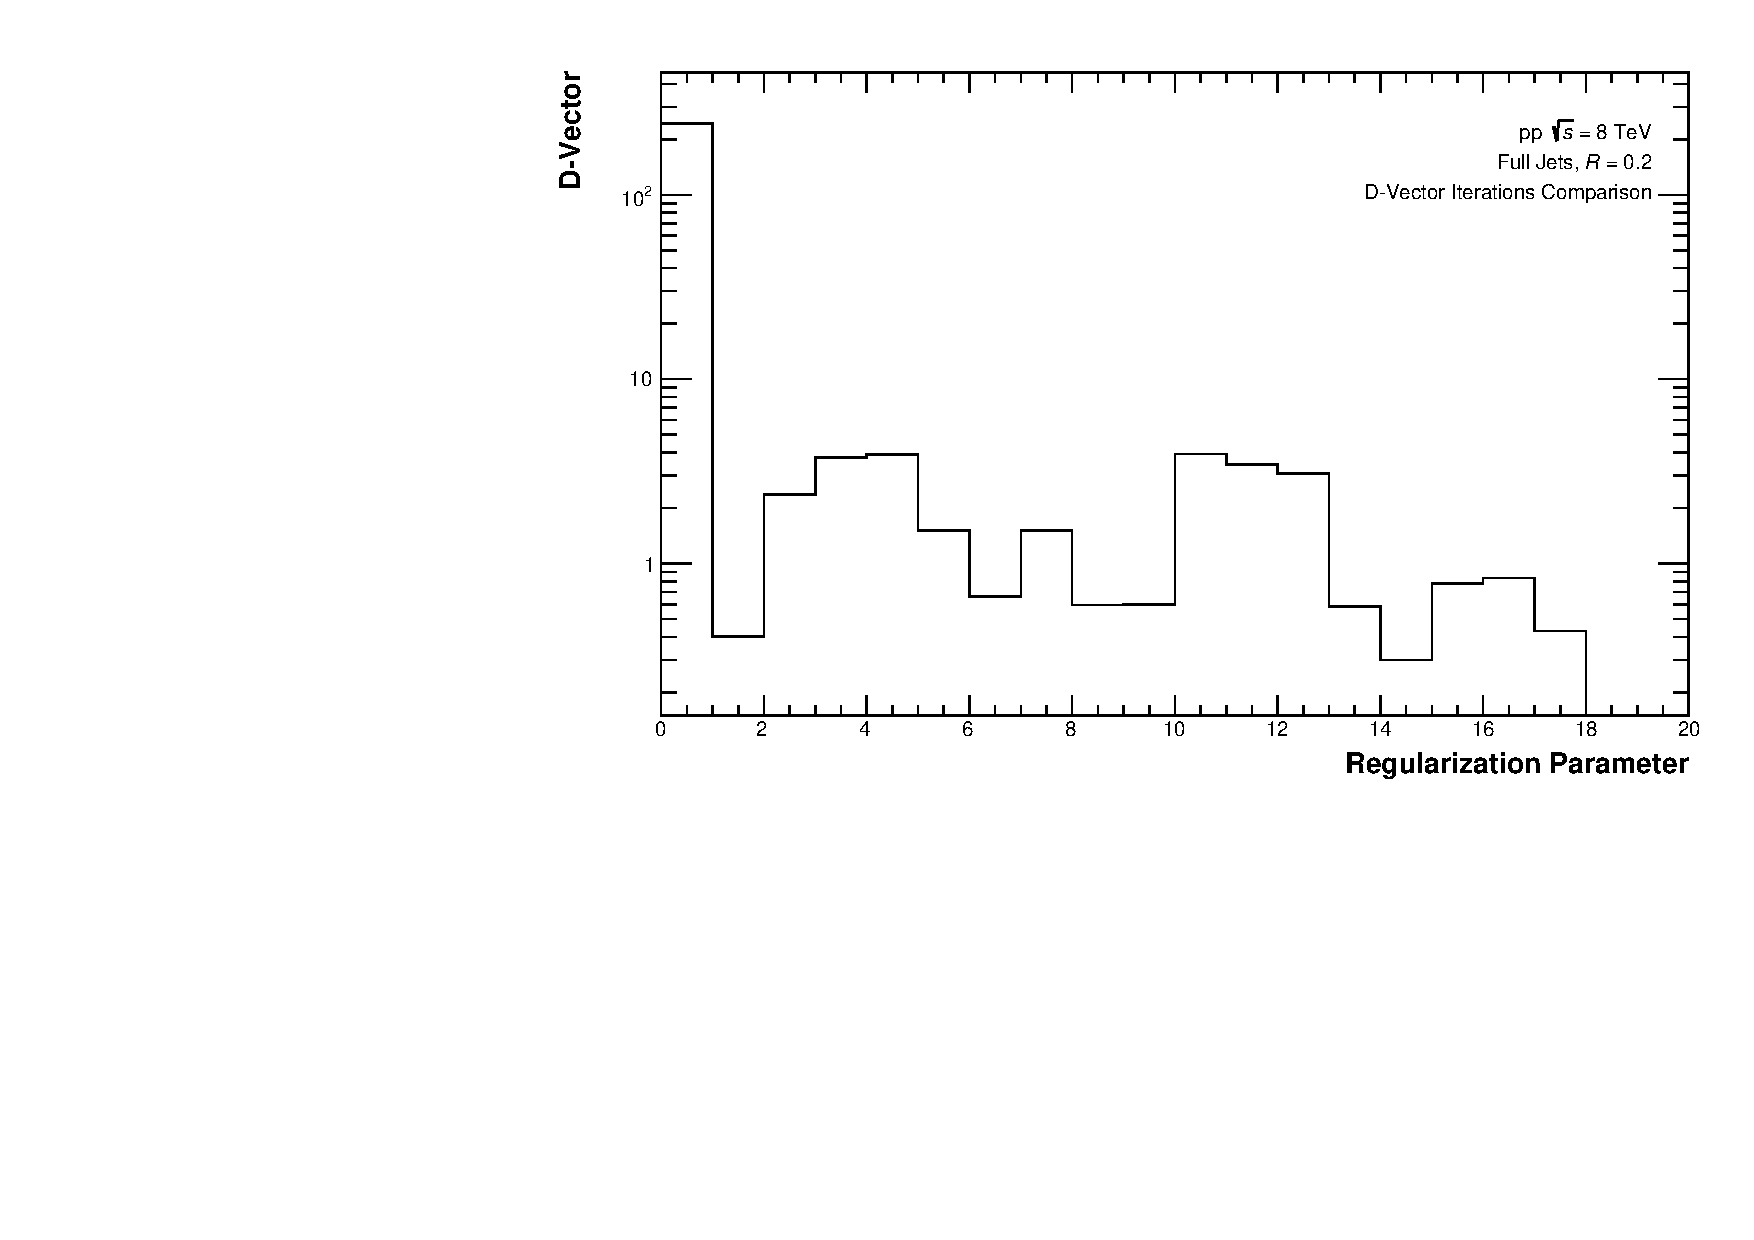
\includegraphics[width=15cm]{figures/DVector/DVector_R02.pdf}
    \caption{D-Vector comparison for different iterations.}
    \label{fig:DVector}
\end{figure}

\begin{figure}
    \centering
    \begin{multicols}{2}
        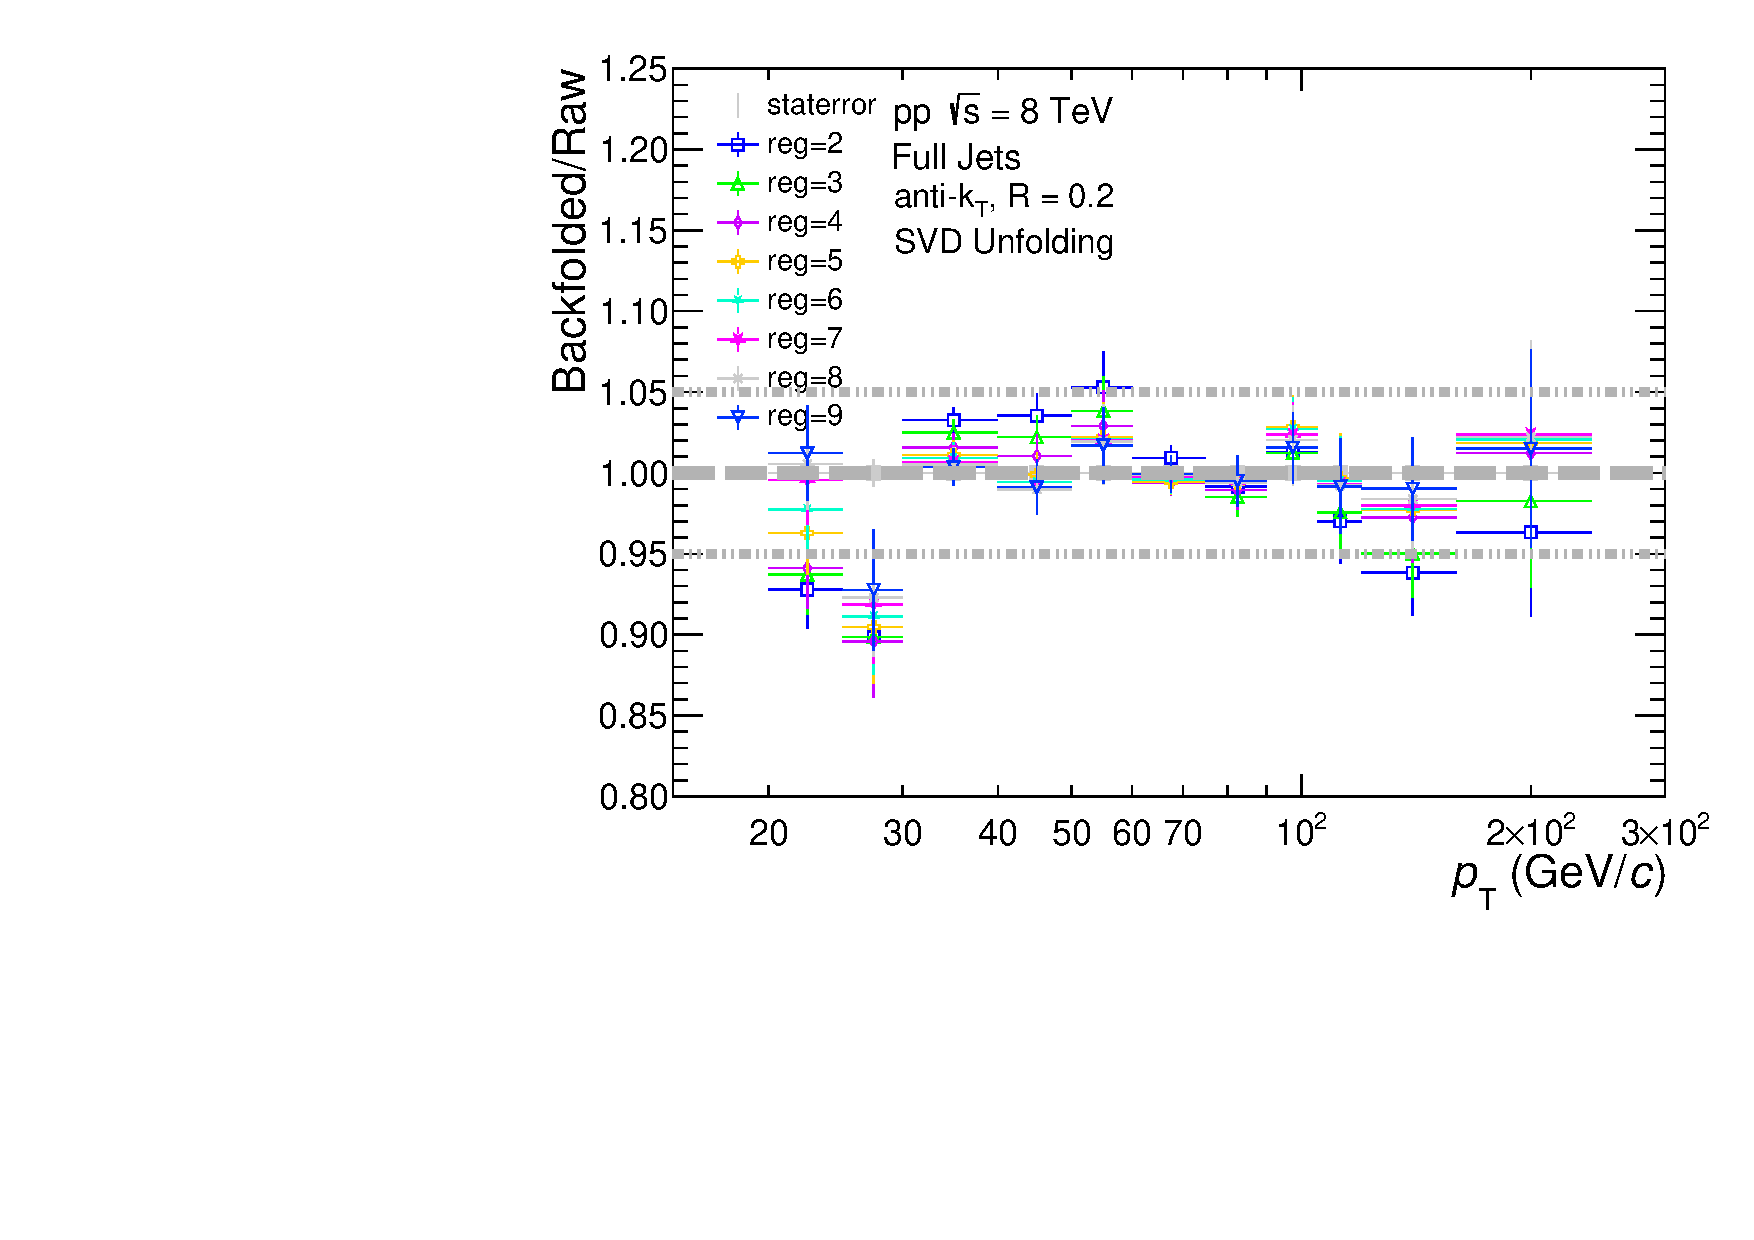
\includegraphics[width=7.5cm]{figures/UnfoldingComparisons/BackfoldedVsRaw/RatioFoldRawSvd_R02.pdf}
    \vfill\null
    \columnbreak
        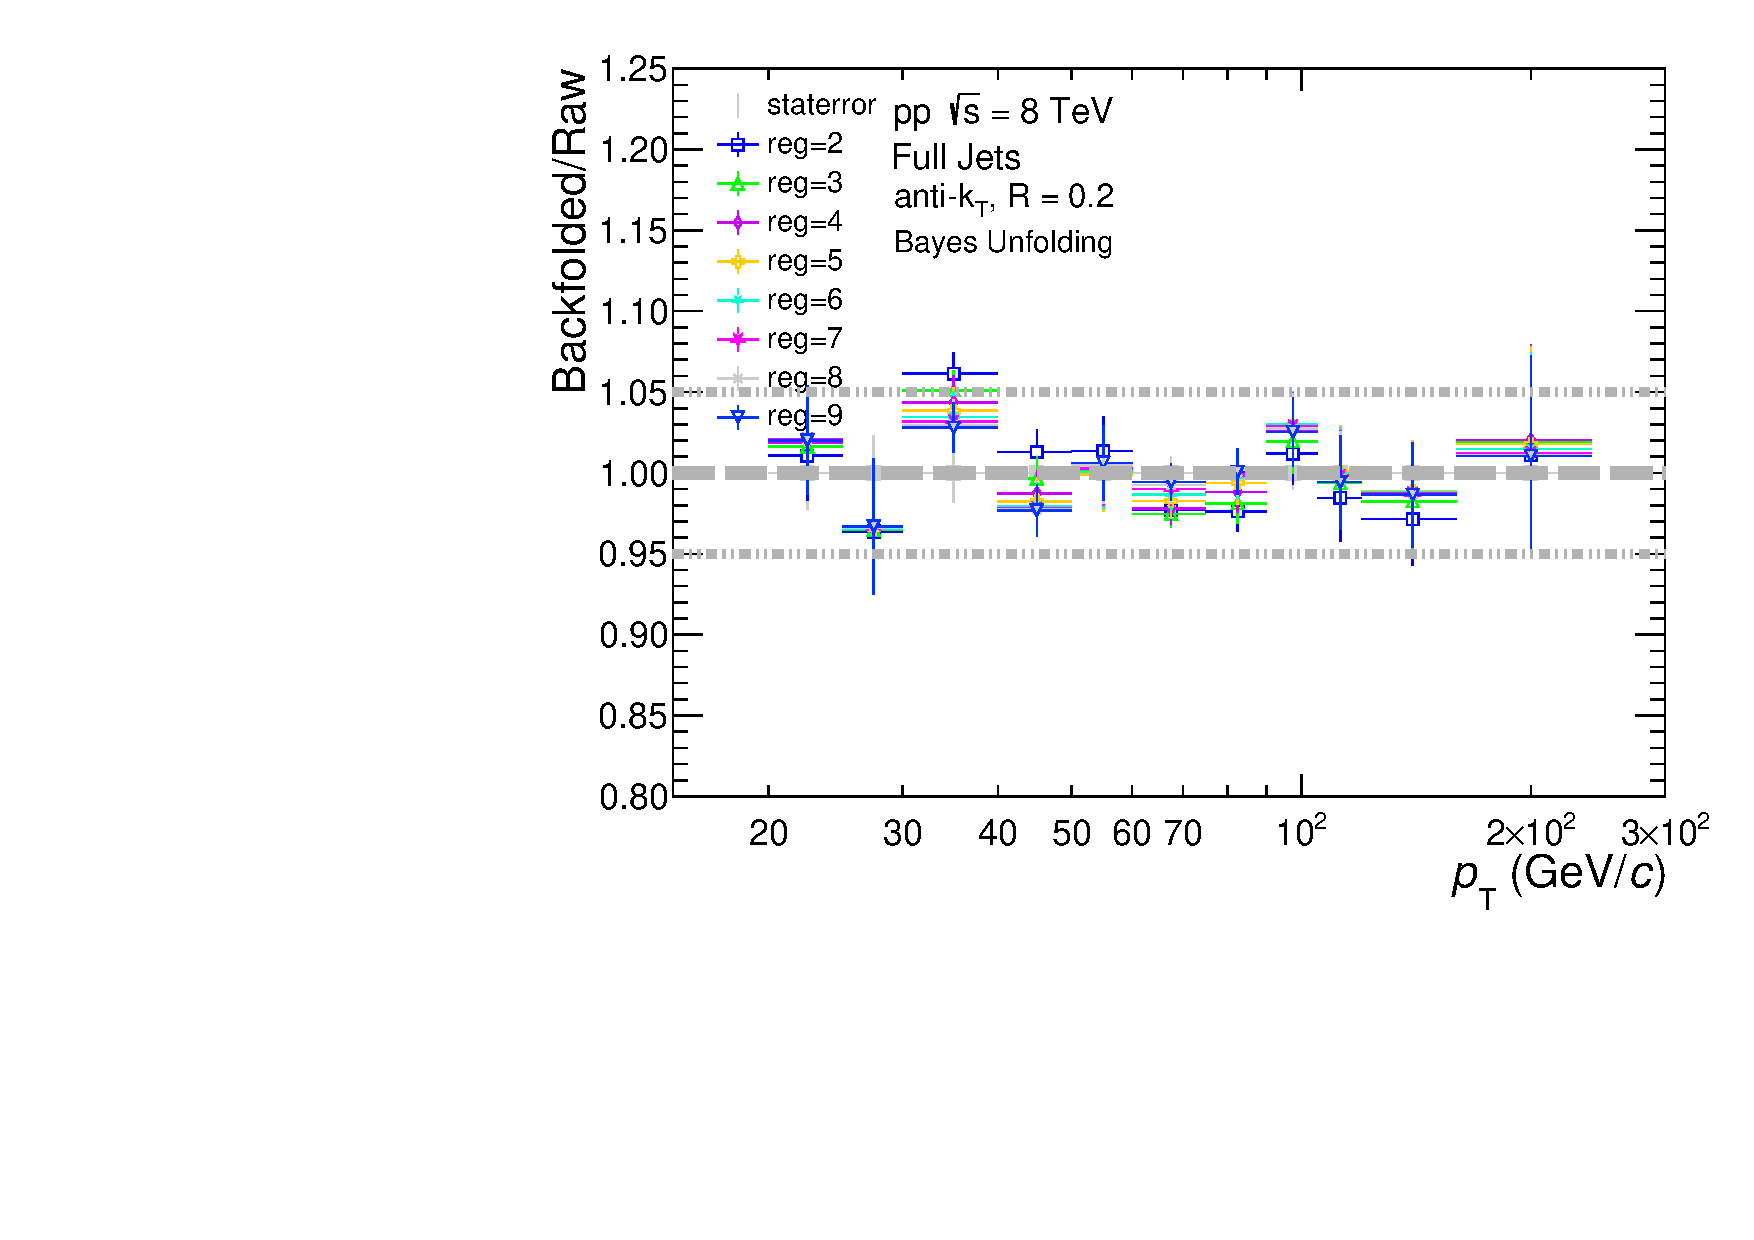
\includegraphics[width=7.5cm]{figures/UnfoldingComparisons/BackfoldedVsRaw/RatioFoldRawBayes_R02.pdf}
        \vfill\null
    \end{multicols}
    \caption{Backfolded vs. Raw for R=0.2.}
    \label{fig:BackfoldedRaw}
\end{figure}

Fig. \ref{fig:BackfoldedRaw} shows the comparison of the back-folded spectrum to the raw spectrum for several regularizations for SVD and bayesian unfolding. Using the default settings for regularization and number of iterations the two unfolding methods produce consistent results. For the largest jet radius some oscillating behavior can be seen. The difference between the unfolding methods is accounted for as systematic uncertainty.

\begin{figure}
    \centering
    \begin{multicols}{2}
            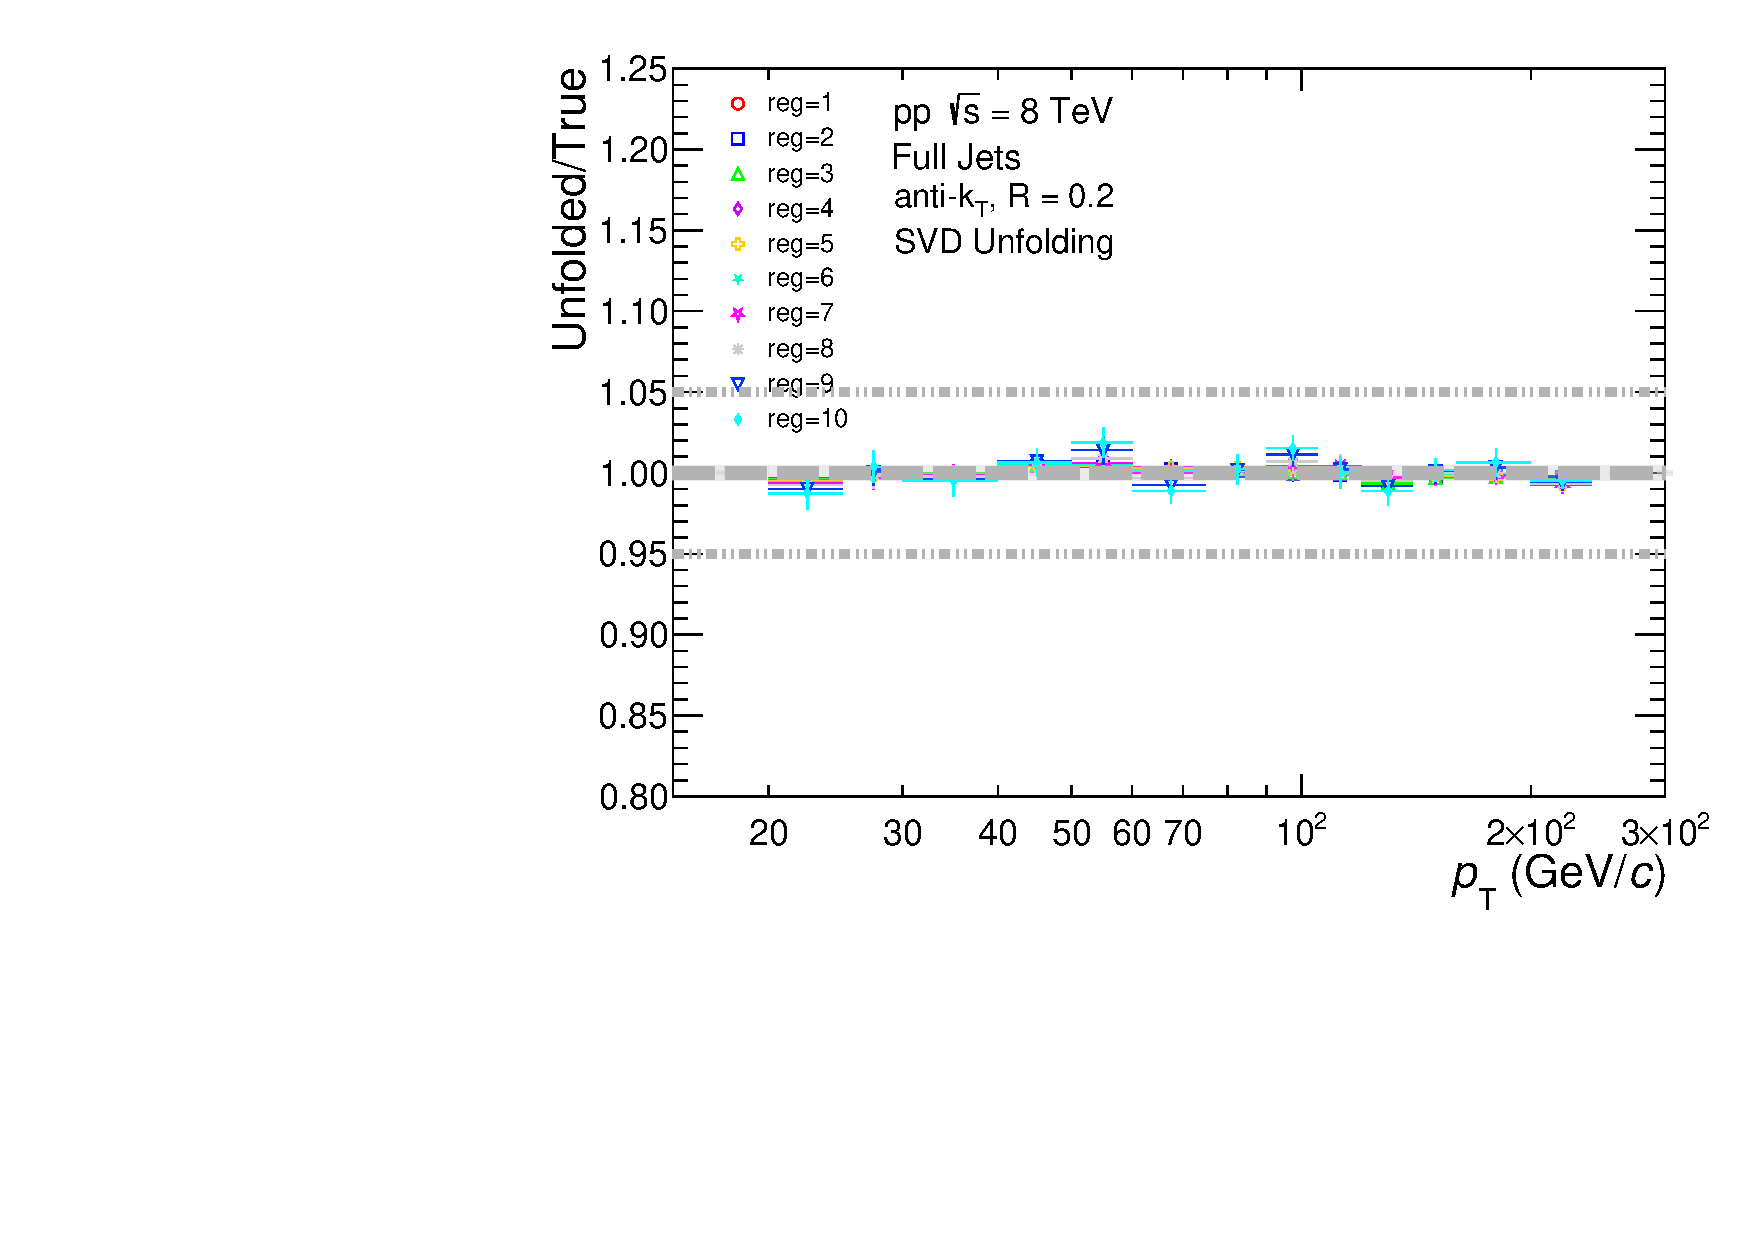
\includegraphics[width=7.5cm]{figures/UnfoldingComparisons/Closure/RatioClosure1DSvd_R02.pdf}
        \vfill\null
        \columnbreak
            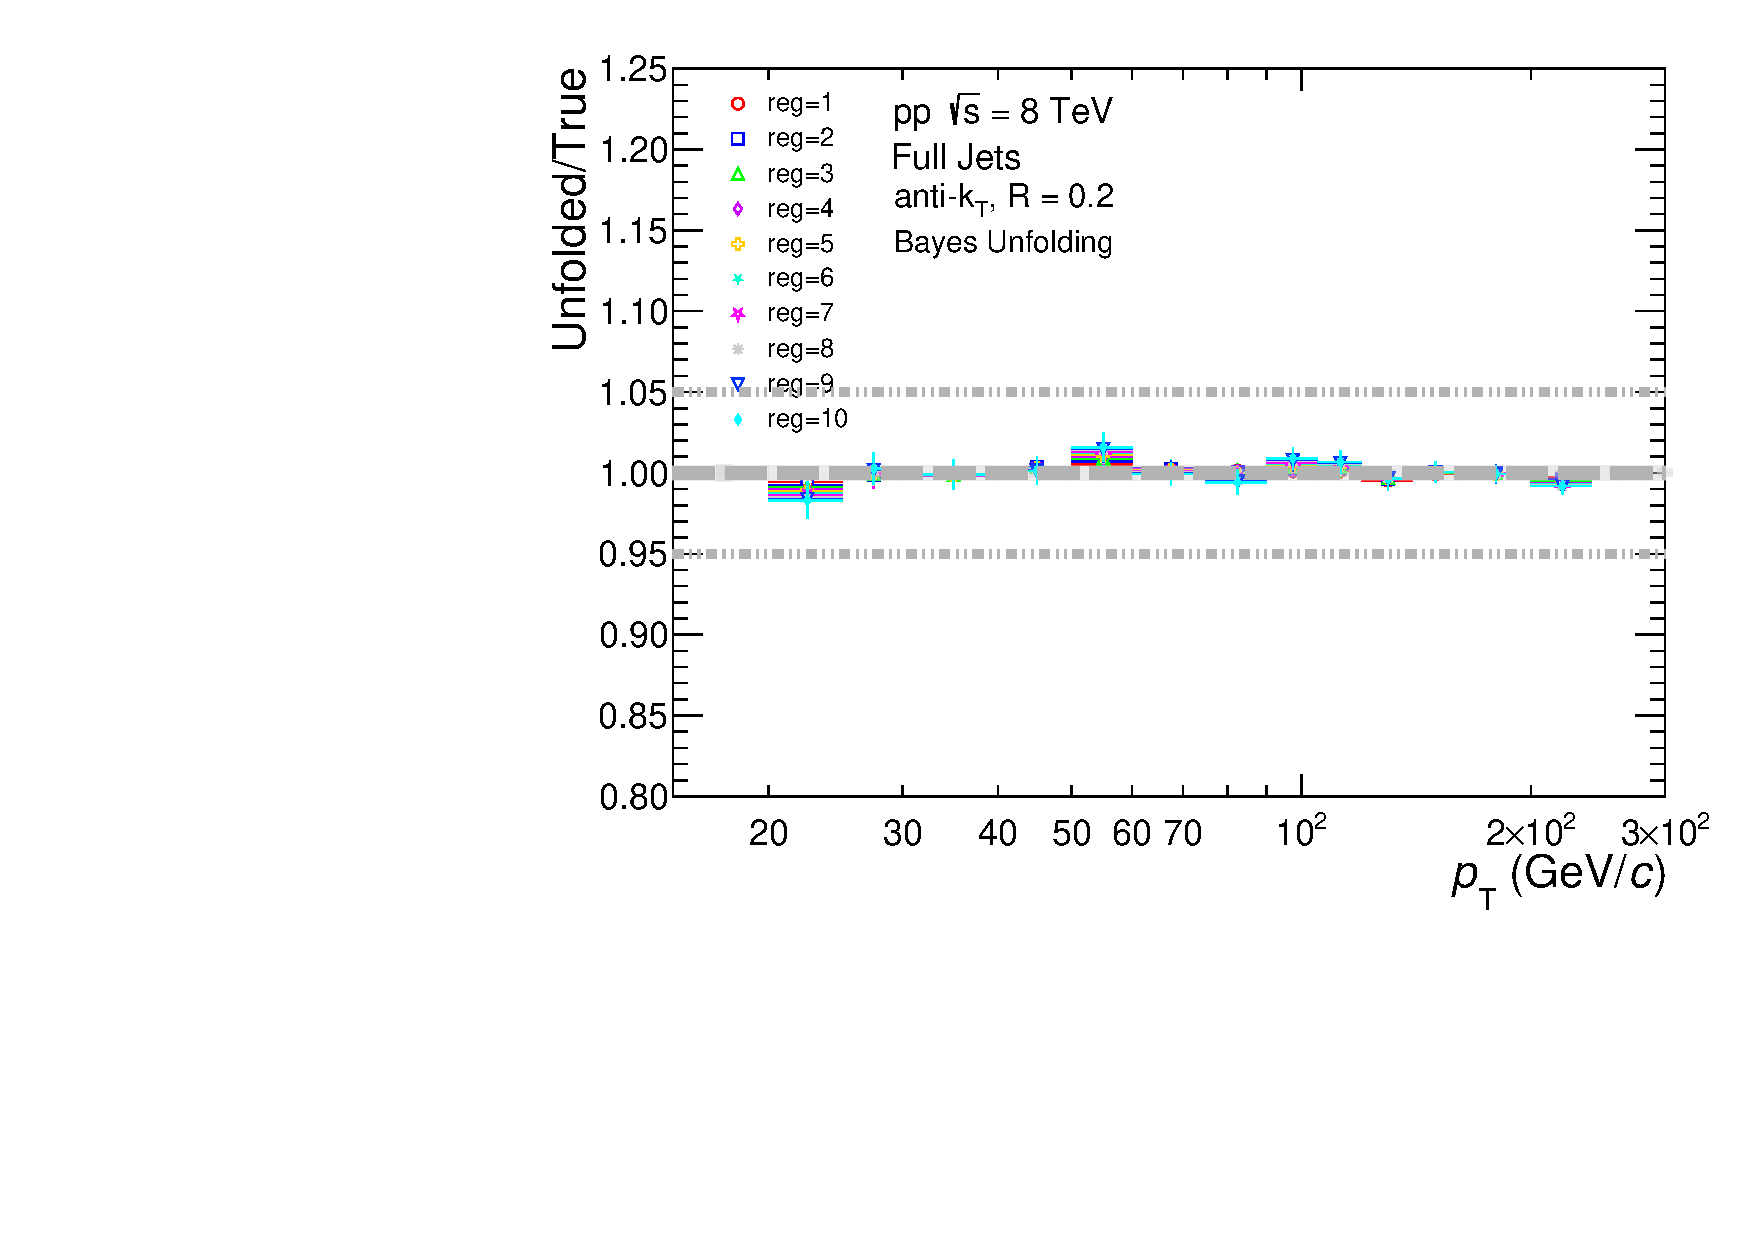
\includegraphics[width=7.5cm]{figures/UnfoldingComparisons/Closure/RatioClosure1DBayes_R02.pdf}
        \vfill\null
    \end{multicols}
    \caption{Closure test for R=0.2.}
    \label{fig:Closure}
\end{figure}

Fig. \ref{fig:Closure} shows the MC closure test for SVD and bayesian unfolding, where the MC sample is split randomly, with 20$\%$ used for the smeared spectrum, and 80$\%$ used for the response matrix. Good agreement between the true spectrum and the unfolded solution is found.

\subsubsection{Unfolding tests - \pPb}

The following plots contain the same unfolding tests for the \pPb dataset. Fig. \ref{fig:RegIterpPb} shows the dependence on the regularization parameter. Fig. \ref{fig:BackfoldedRawpPb} shows the comparison of the back-folded to the raw spectrum. Fig. \ref{fig:ClosurepPb} shows the MC closure tests. Fig. \ref{fig:DVectorpPb} shows the D-vector analysis. Appendix \ref{sec:AppendixUnfoldingTestspPb} contains the remaining jet radii. Bayesian unfolding shows better stability, and is used as the default unfolding method.

\begin{figure}
    \centering
    \begin{multicols}{2}
            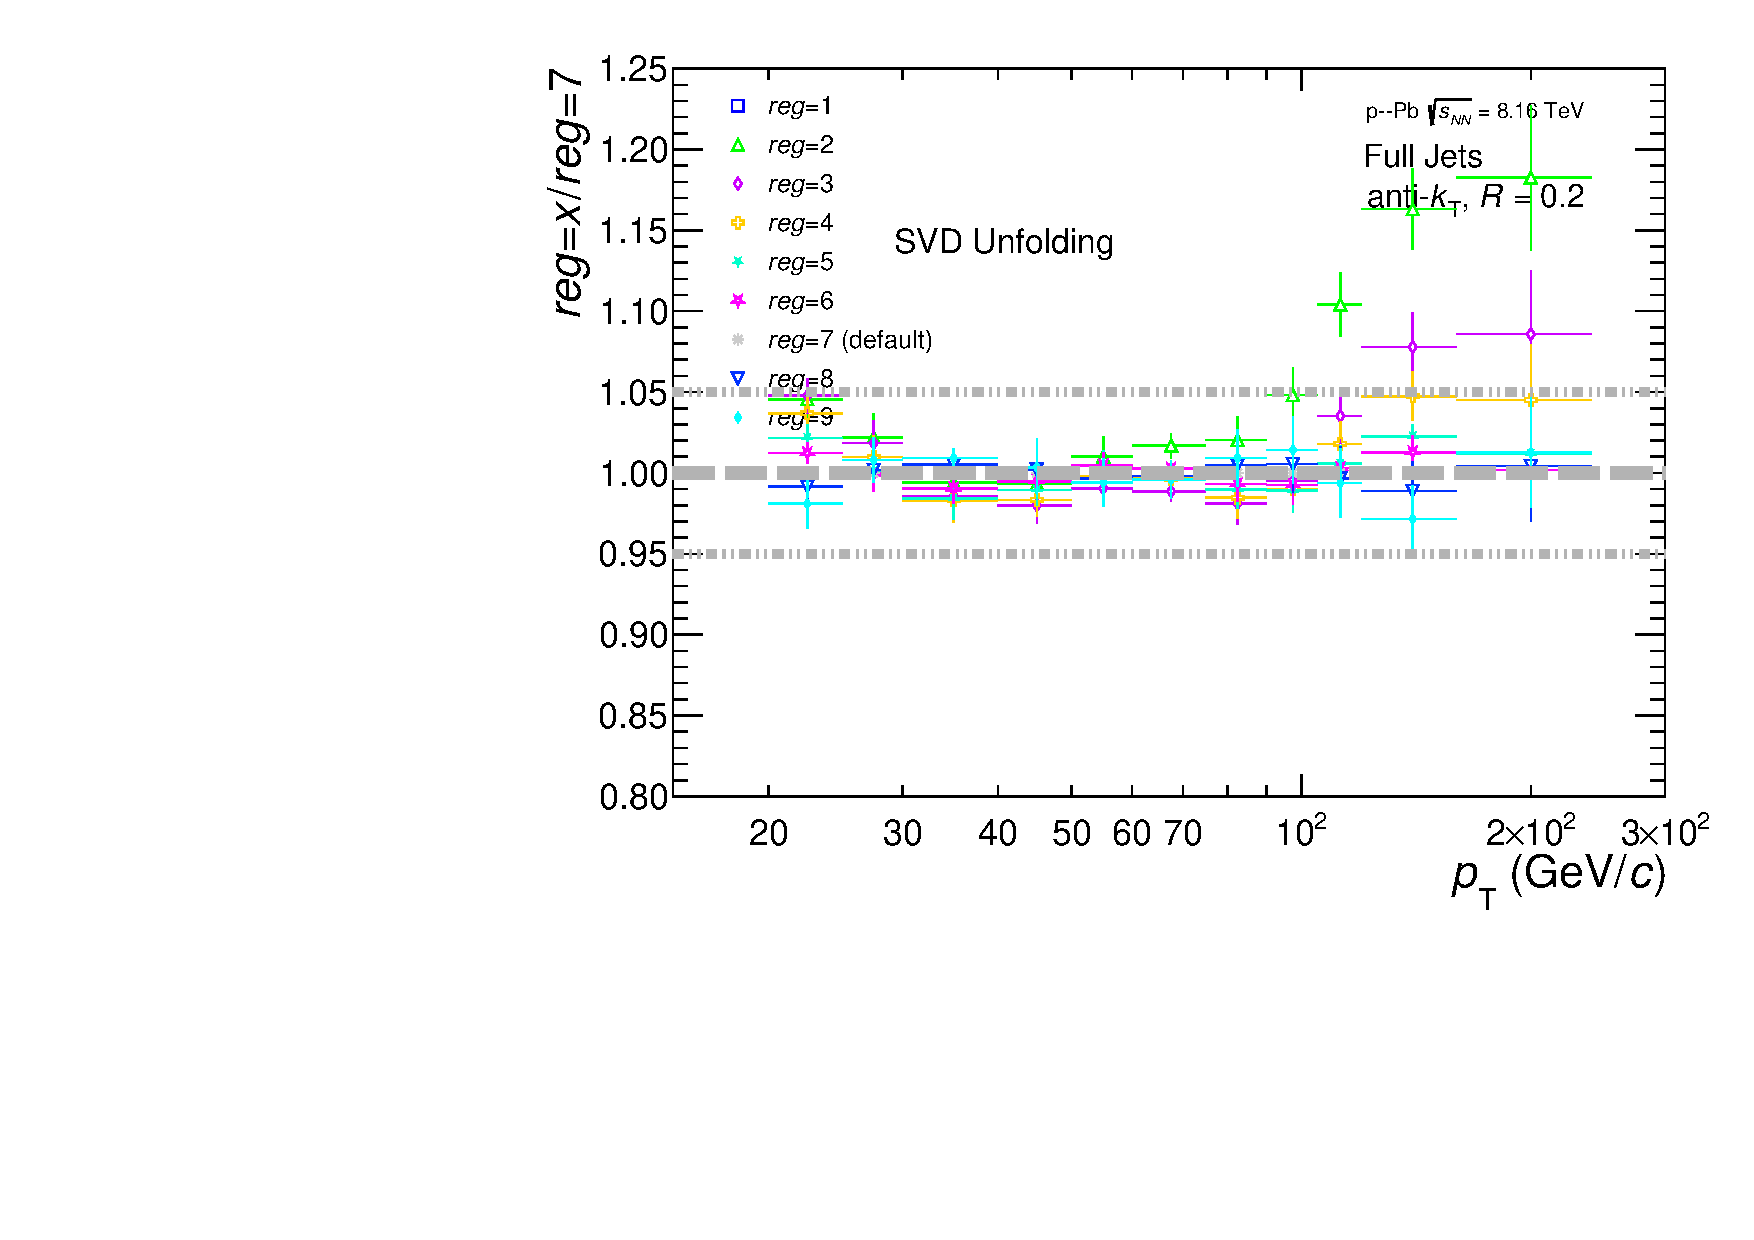
\includegraphics[width=7.5cm]{figures/pPbFigures/UnfoldingComparisons/Regularizations/RatioRegularizationSvd_R02.pdf}
        \vfill\null 
        \columnbreak
            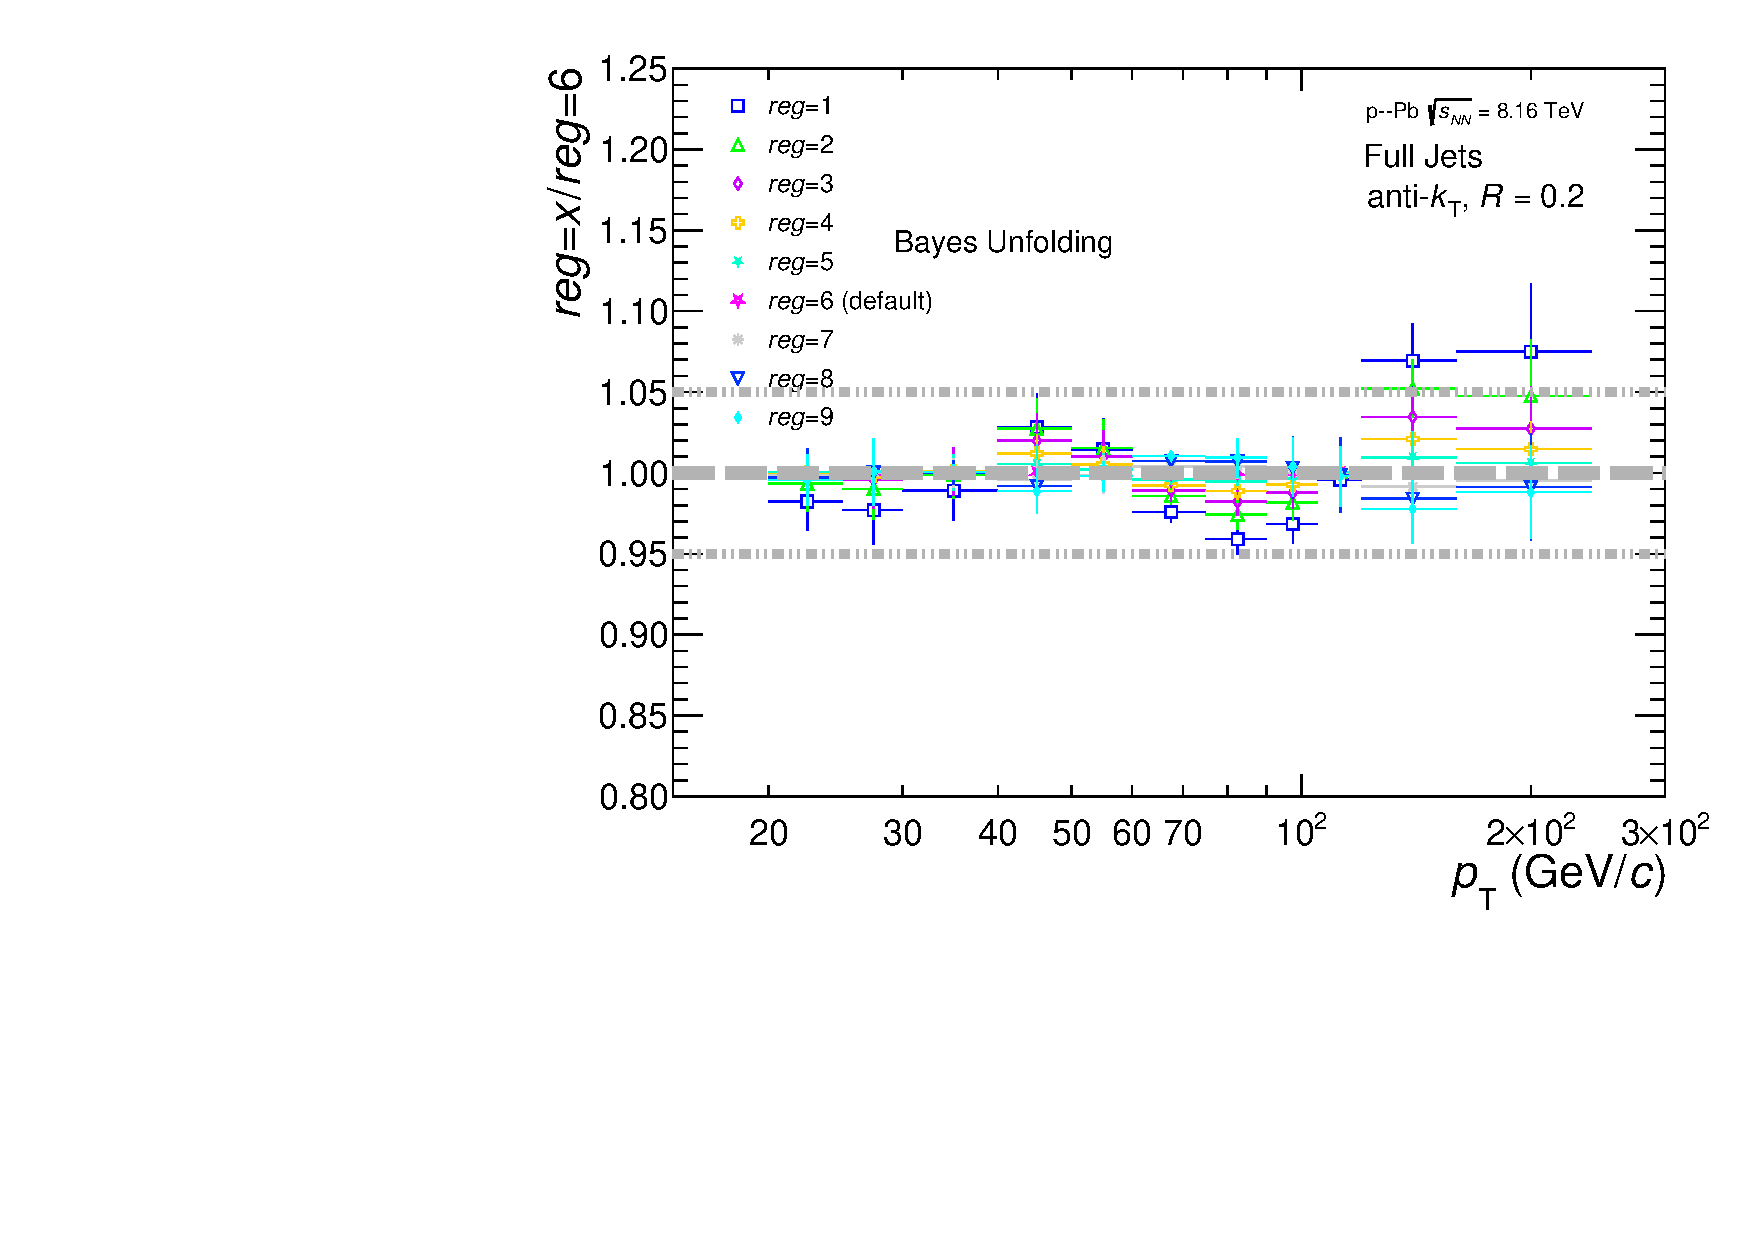
\includegraphics[width=7.5cm]{figures/pPbFigures/UnfoldingComparisons/Regularizations/RatioRegularizationBayes_R02.pdf}
        \vfill\null
    \end{multicols}
    \caption{Regularization dependence for SVD (left) and Bayesian (right) unfolding.}
    \label{fig:RegIterpPb}
\end{figure}

\begin{figure}
    \centering
    \begin{multicols}{2}
        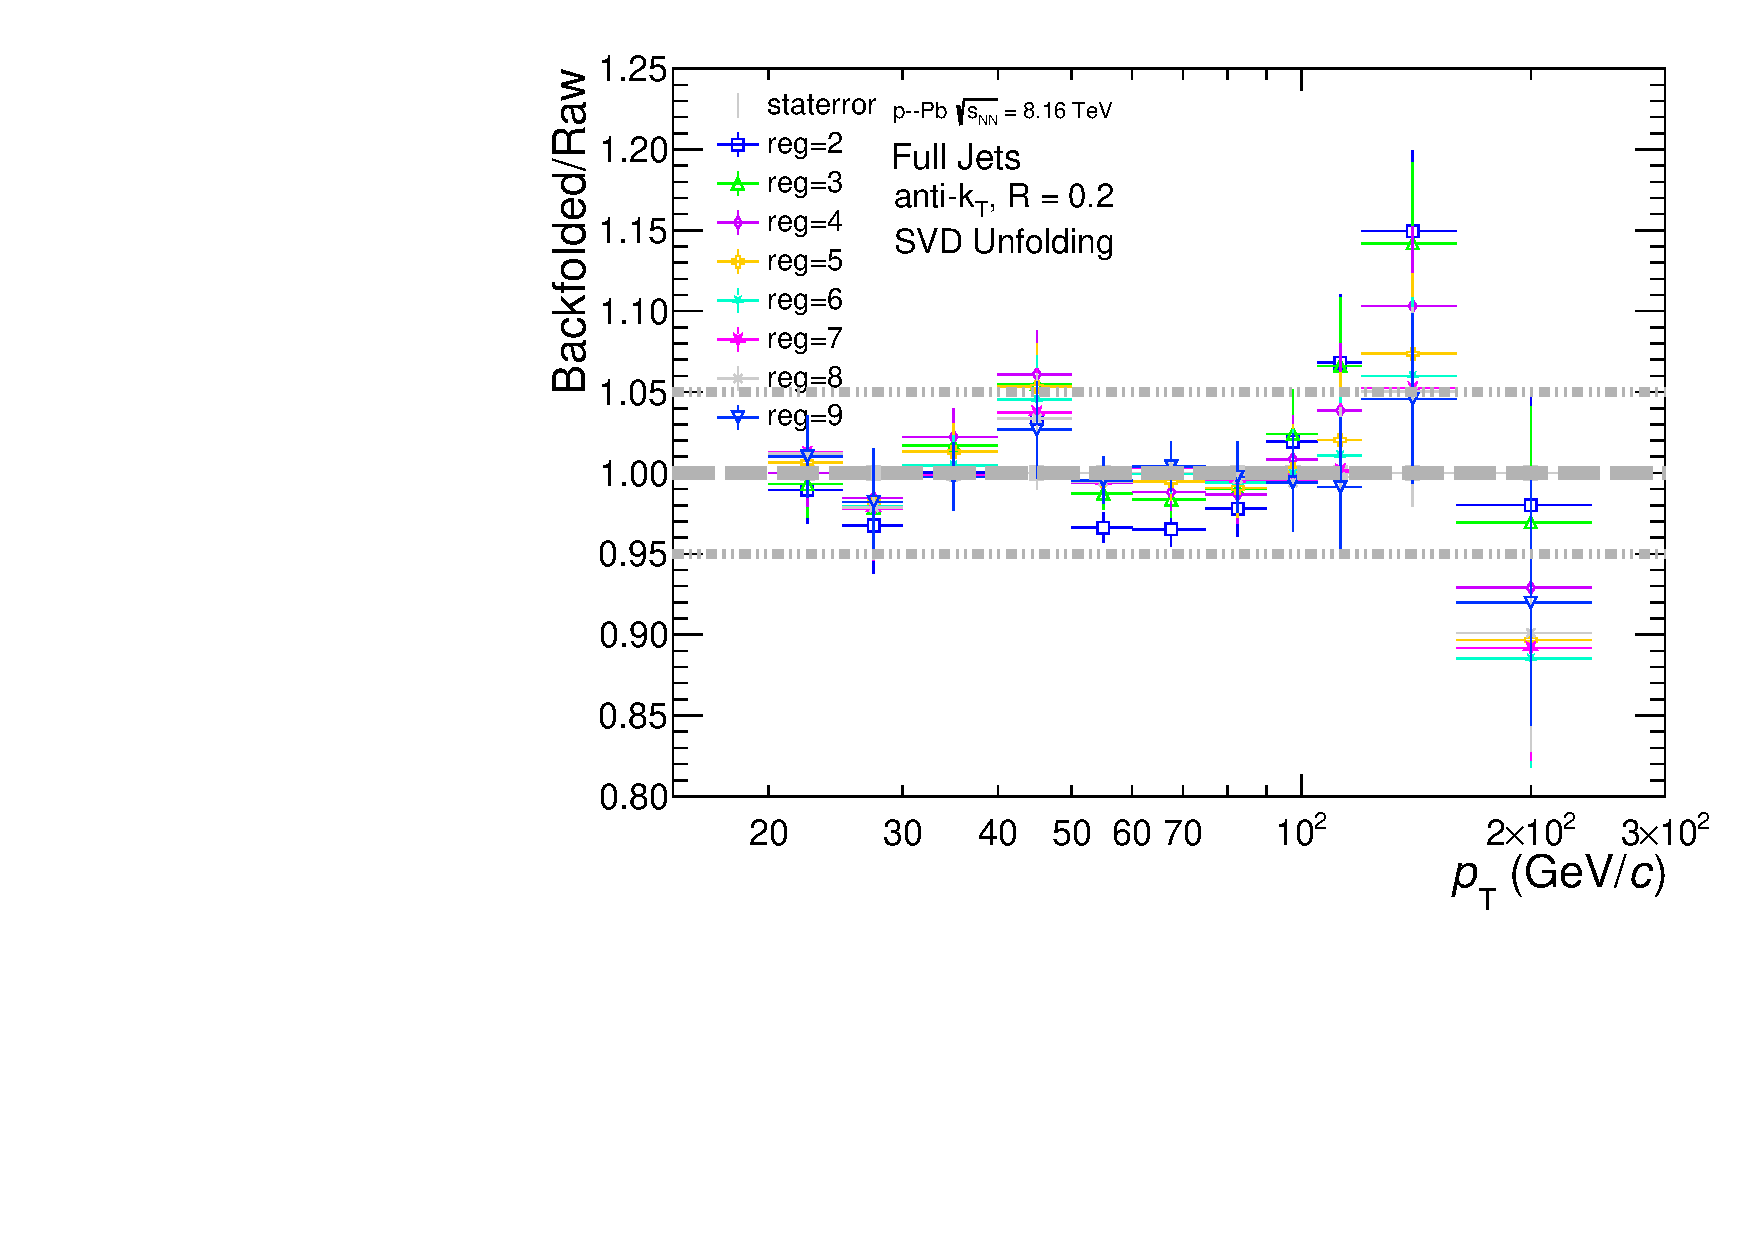
\includegraphics[width=7.5cm]{figures/pPbFigures/UnfoldingComparisons/BackfoldedVsRaw/RatioFoldRawSvd_R02.pdf}
    \vfill\null
    \columnbreak
        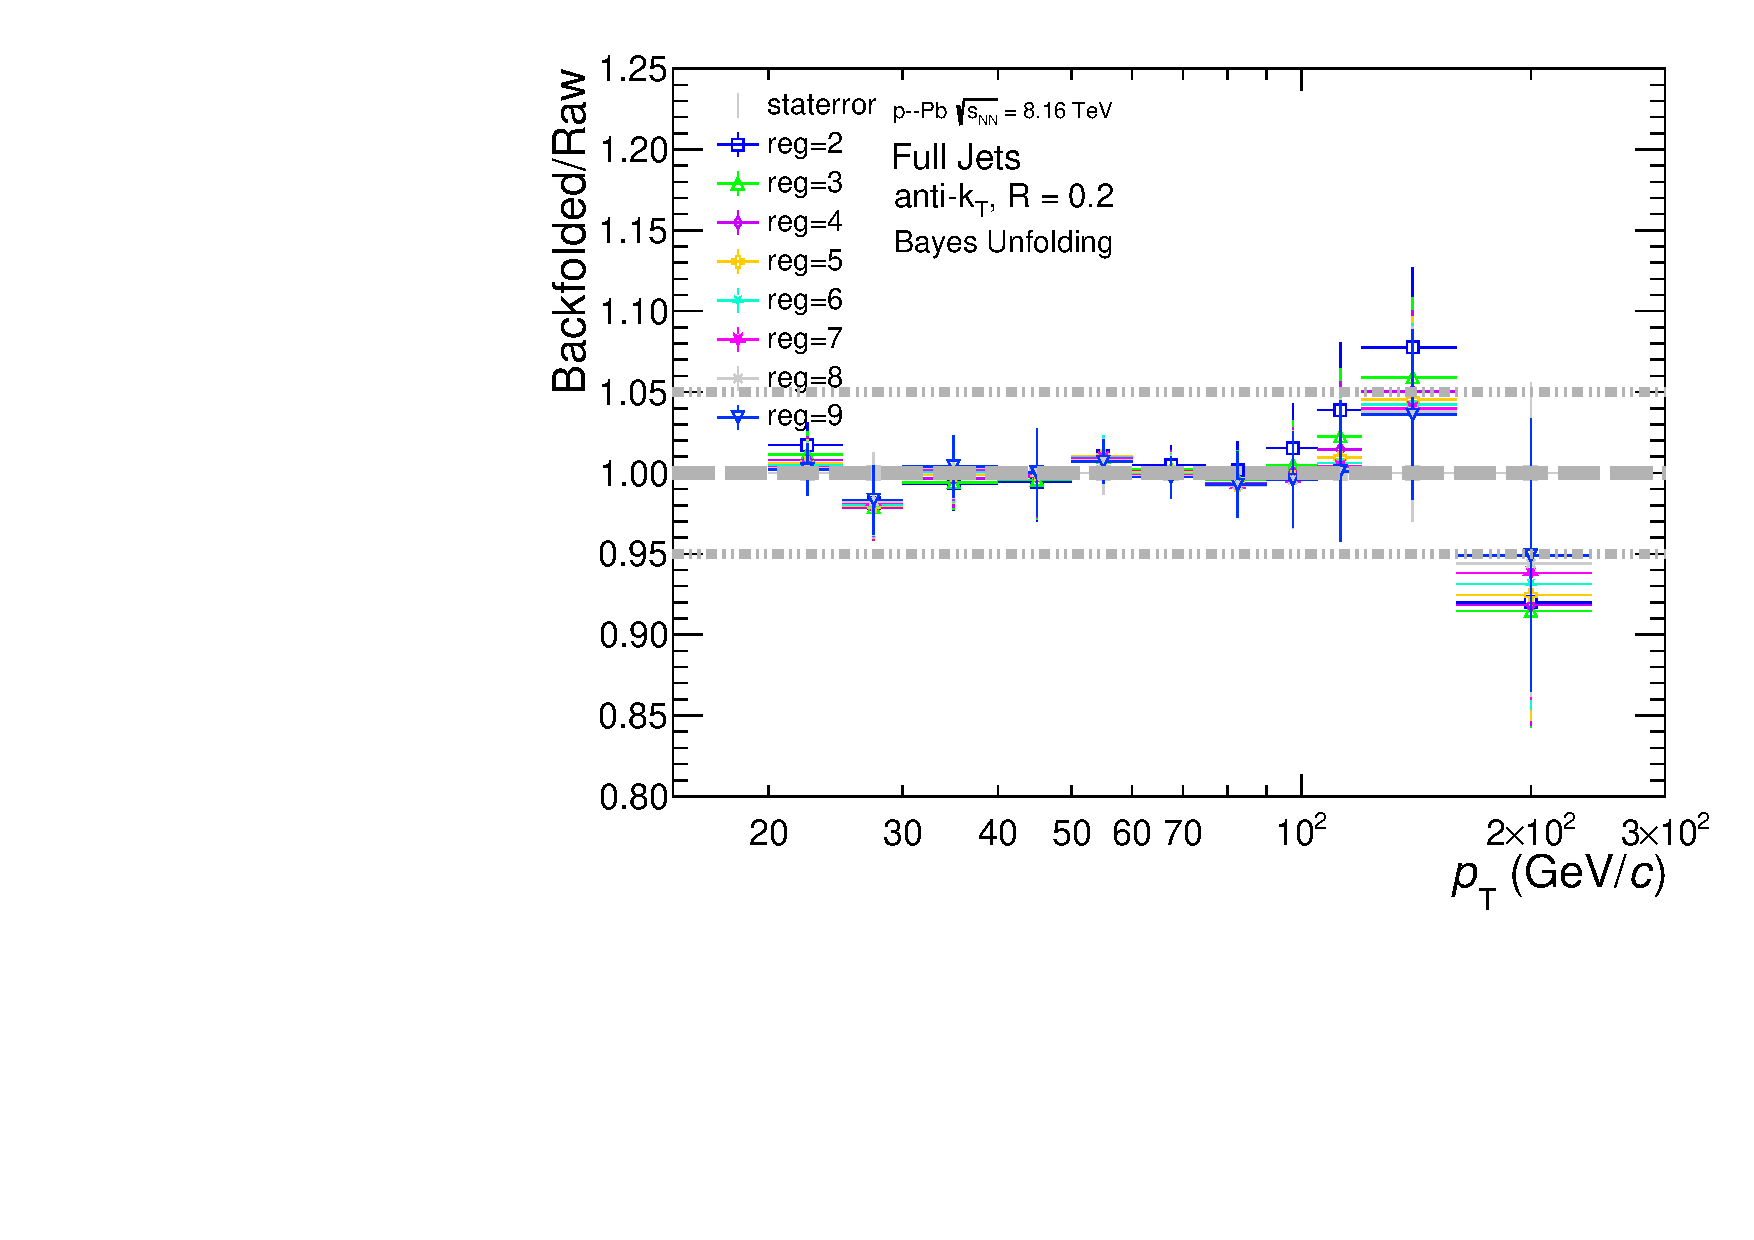
\includegraphics[width=7.5cm]{figures/pPbFigures/UnfoldingComparisons/BackfoldedVsRaw/RatioFoldRawBayes_R02.pdf}
        \vfill\null
    \end{multicols}
    \caption{Backfolded vs. Raw for R=0.2.}
    \label{fig:BackfoldedRawpPb}
\end{figure}

\begin{figure}
    \centering
    \begin{multicols}{2}
            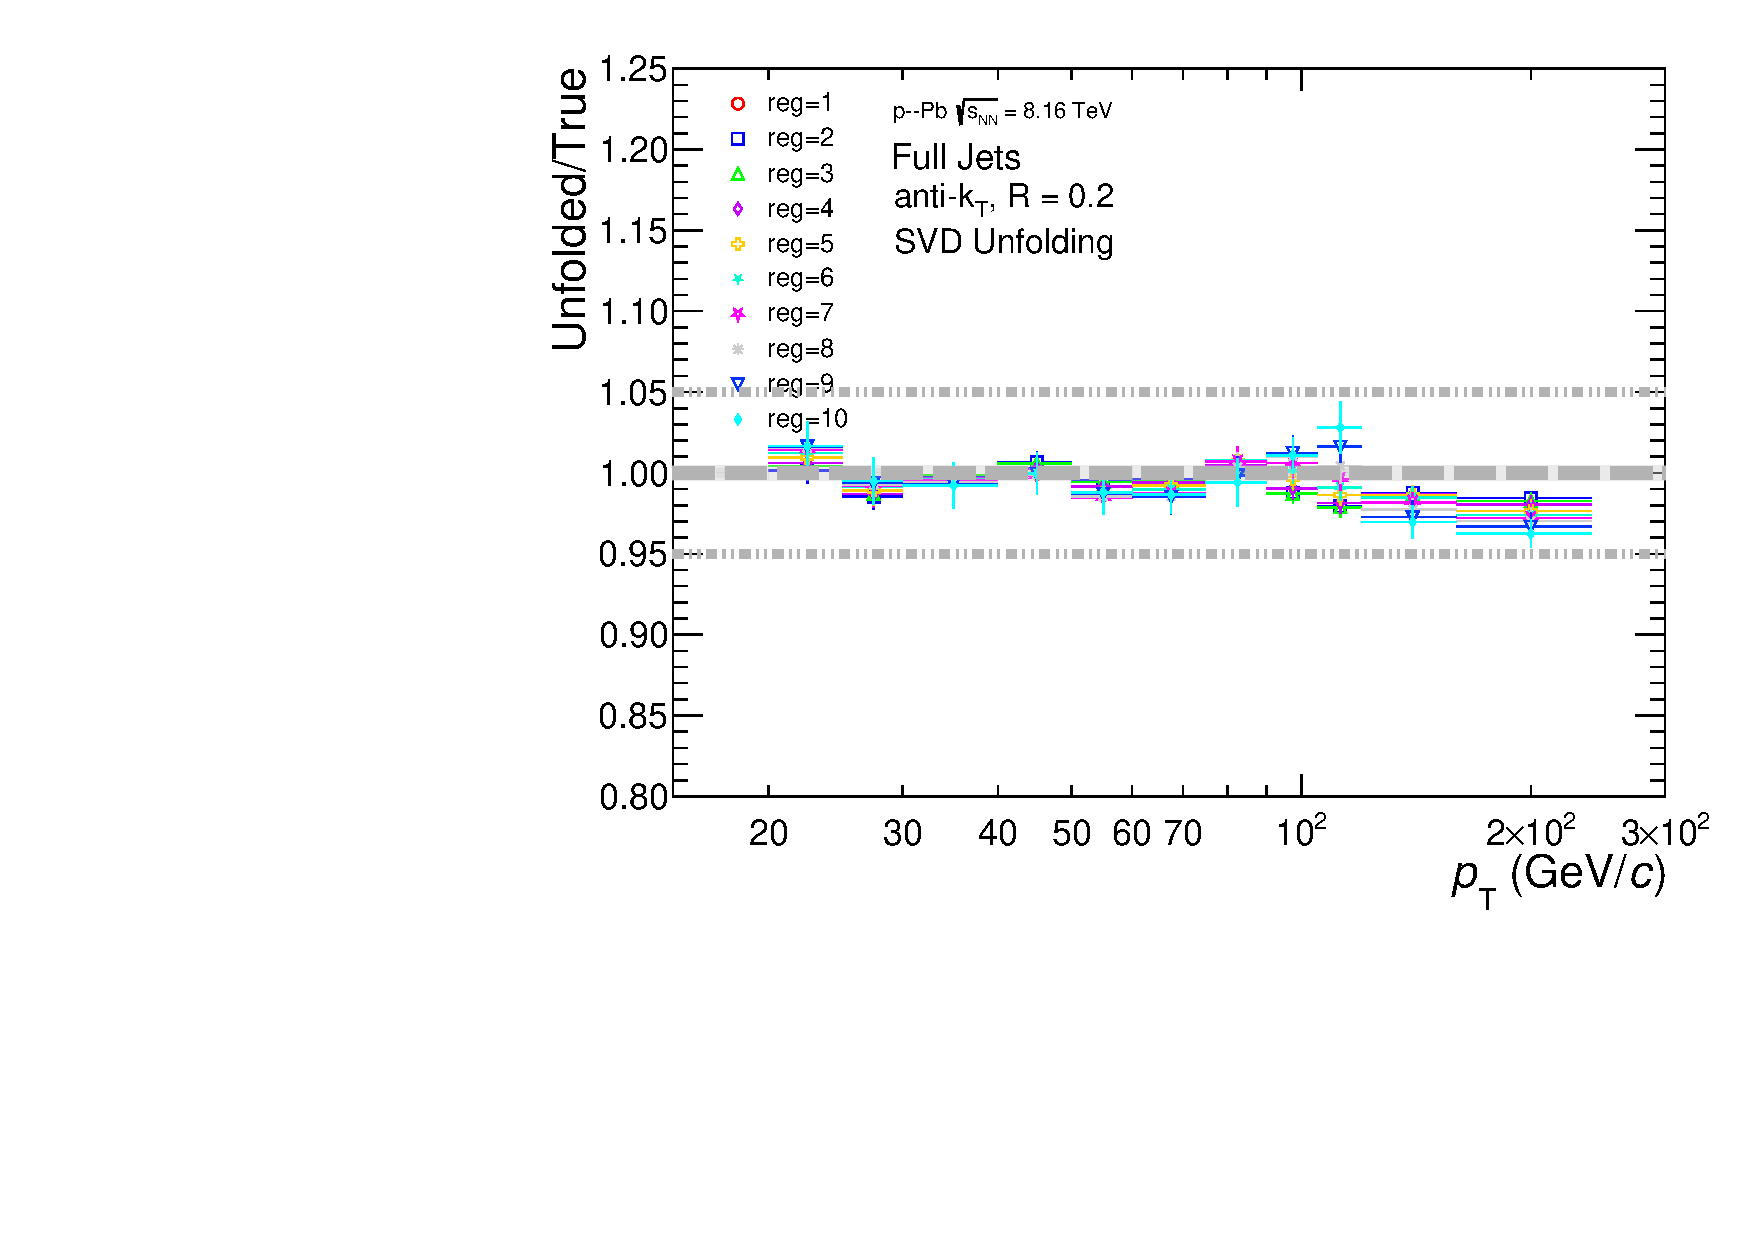
\includegraphics[width=7.5cm]{figures/pPbFigures/UnfoldingComparisons/Closure/RatioClosure1DSvd_R02.pdf}
        \vfill\null
        \columnbreak
            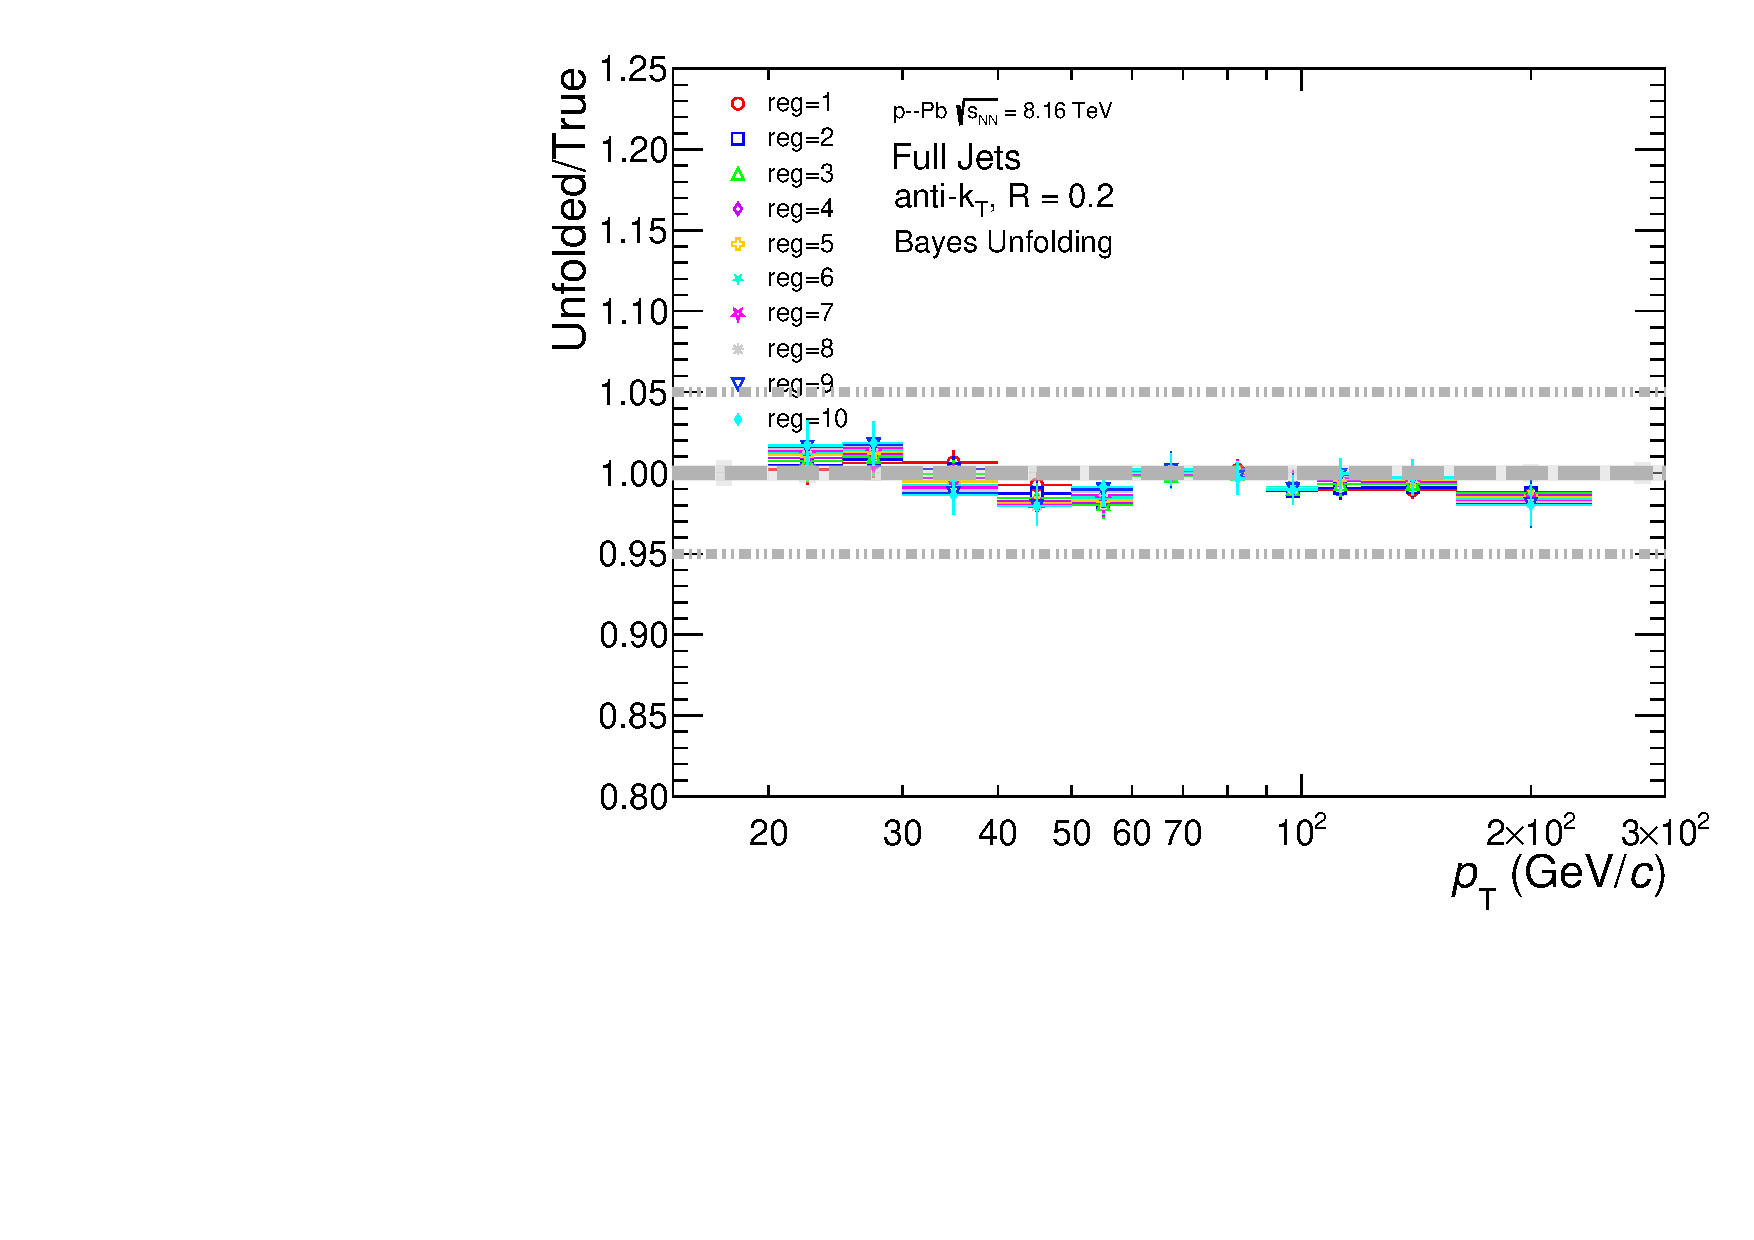
\includegraphics[width=7.5cm]{figures/pPbFigures/UnfoldingComparisons/Closure/RatioClosure1DBayes_R02.pdf}
        \vfill\null
    \end{multicols}
    \caption{Closure test for R=0.2.}
    \label{fig:ClosurepPb}
\end{figure}

\begin{figure}
    \centering
    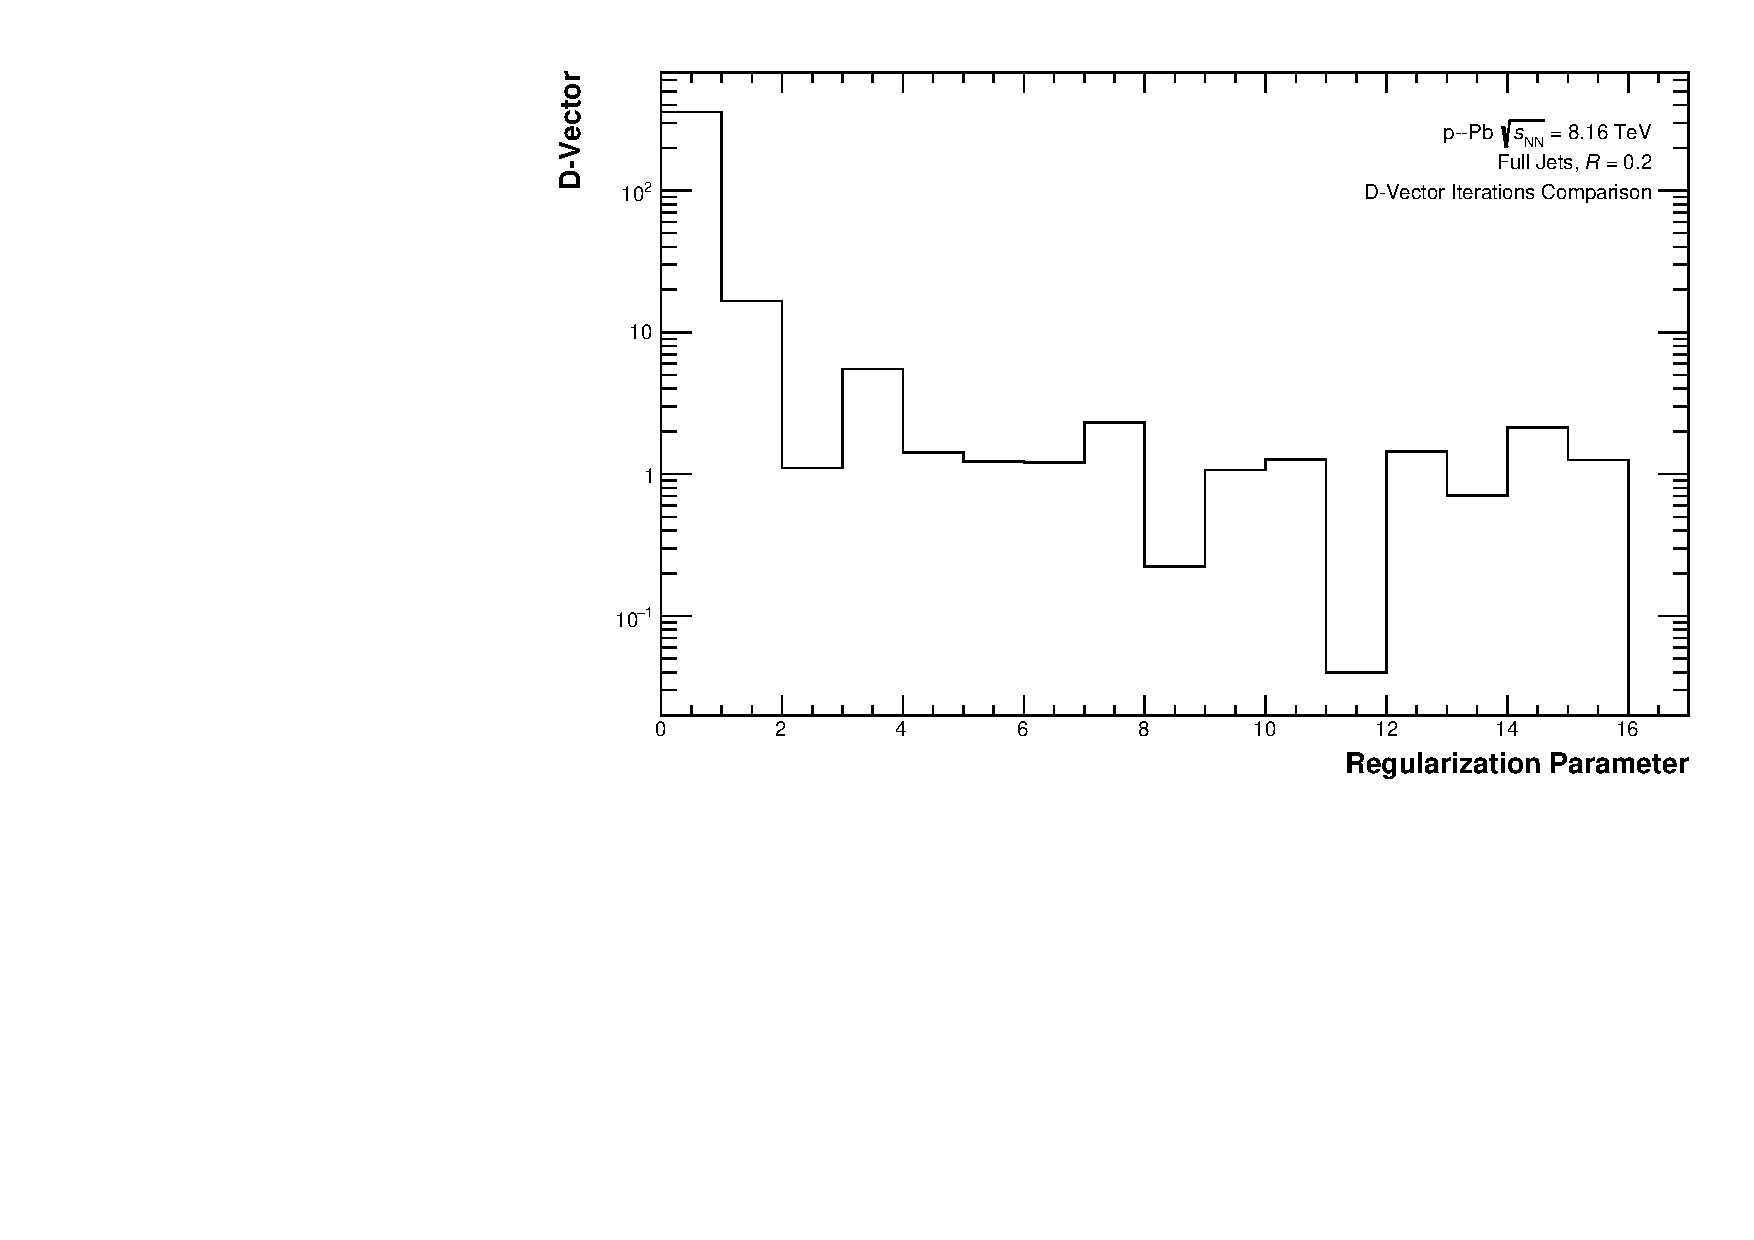
\includegraphics[width=15cm]{figures/pPbFigures/DVector/DVector_R02.pdf}
    \caption{D-Vector comparison for different iterations.}
    \label{fig:DVectorpPb}
\end{figure}

\subsection{Study of a bias the spectrum at high-\texorpdfstring{\pT}{pT} due to possible fake contributions}
\label{sec:biasStudy}

The track sample at high-\pT is contaminated by fake tracks, originating either from a misreconstruction of the \pT of tracks with lower momenta, or from a contamination of tracks from muons from cosmic or atmospheric sources passing the detector in coincidence with triggered events. A study was done to account for these fake tracks and can be found in \cite{anaNoteMFasel}.